% per commentare una riga mettere % al suo inizio
% per s-commentare una riga (ossia attivarla) togliere il % al suo inizio
%
\documentclass[cucitura%lascia margine per la rilegatura
%,twoside% per stampa fronte-retro (fortemente consigliato per tesi voluminose, opzionale per le altre)
,12pt% font più grande (12pt) rispetto a quello normalmente usato (11pt)
]{toptesi}
%
% Cambiare encoding a piacere; oppure non caricare nessun encoding se si usano
% solo caratteri a 7 bit (ASCII) nei file d'entrata.
%
\usepackage[a-1b]{pdfx}% formato PDF/A, obbligatorio per l'archiviazione delle tesi di Polito
\usepackage[utf8]{inputenc}% IMPORTANTE! usare codifica UTF-8 per le lettere accentate
\usepackage{amsmath, amssymb}
\usepackage{nccmath}
\usepackage{appendix}
\usepackage{longtable}
\usepackage{lscape}
\usepackage{adjustbox}
\usepackage{float}
\usepackage{accsupp}
\usepackage{pgfplots}
%
% Commentare le righe seguenti se NON si è specificata l'opzione "pdfa"
\hypersetup{%
    pdfpagemode={UseOutlines},
    bookmarksopen,
    pdfstartview={FitH},
    colorlinks,
    linkcolor={blue},
    citecolor={red},
    urlcolor={blue}
  }
% \documentclass[11pt,twoside,oldstyle,autoretitolo,classica,greek]{toptesi}
% \usepackage[or]{teubner}
%%%%%%%%%%%%%%%%%%%%%%%%%%%%%%%%%%%%%%%%%%%%%%%%%%%%
%


% per inserire uno spazio "fantasma" nella definizione di un'abbreviazione
\usepackage{xspace}

% per inserire un DOI senza problemi coi caratteri "strani" ivi presenti
\usepackage{doi}
\renewcommand{\doitext}{DOI }% originally was "doi:"

% per inserire correttamente le unità di misura SI (incluse quelle binarie)
\usepackage[binary-units]{siunitx}
% se si desidera usare / invece che la potenza -1 per indicare "al secondo"
\sisetup{per-mode=symbol}

% per inserire codice di programmazione complesso
\usepackage{listings}% per inserire codice di programmazione complesso
\lstset{
basicstyle=\ttfamily,
columns=fullflexible,
xleftmargin=3ex,
numbers=none,
breaklines,
breakatwhitespace,
escapechar=`
}

% modify some page parameters
\setlength{\parskip}{\medskipamount}
\advance\voffset -5mm
\advance\textheight 30mm

% riga orizzontale
\newcommand{\HRule}{\rule{\linewidth}{0.2mm}}
% esempio di creazione di semplici abbreviazioni
\newcommand{\ltx}{\LaTeX\xspace}
\newcommand{\txw}{TeXworks\xspace}
\newcommand{\mik}{MikTex\xspace}
\newcommand{\html}{HTML\xspace}
\newcommand{\xhtml}{XHTML\xspace}

% esempio di creazione di un'abbreviazione con un parametro (il cui uso è indicato da #1)
\newcommand{\cmd}[1]{\texttt{#1}\xspace}
% per citare un RFC, es. \rfc{822}
\newcommand{\rfc}[1]{RFC-#1\xspace}
% per citare un file (es. \file{autoexec.bat}) o una URI fittizia (es. \file{http://www.lioy.it/})
% per le URI vere usare \url o \href
\newcommand{\file}[1]{\texttt{#1}\xspace}
% per inserire codice di esempio in-line
\newcommand{\code}[1]{\lstinline|#1|}
% importante per i pathname Windows perché non si può usare \ essendo un carattere riservato di Latex
\newcommand{\bs}{\textbackslash}
% definizione di un termine: formattazione ed inserimento nell'indice
\newcommand{\tdef}[1]{\textit{#1}\index{#1}}
% meta-termine, usato tipicamente nelle definizioni dei tag
\newcommand{\meta}[1]{\textit{#1}}


\definecolor{blond}{rgb}{0.98, 0.94, 0.75}
\definecolor{gray}{rgb}{0.4,0.4,0.4}
\definecolor{darkblue}{rgb}{0.0,0.0,0.6}
\definecolor{cyan}{rgb}{0.0,0.6,0.6}
\definecolor{Maroon}{rgb}{0.5,0.0,0.0}
\definecolor{darkgreen}{rgb}{0.0,0.5,0.0}

%\ExtendCaptions{english}{Abstract}{Acknowledgements}

\lstset{
	numbers=none, 
	numberstyle=\small, 
	numbersep=8pt, 
	frame = single, 
	framexleftmargin=20pt
}

\lstdefinelanguage{XML}
{
	backgroundcolor = \color{blond},
	basicstyle=\ttfamily\footnotesize,
	morestring=[b]",
	moredelim=[s][\bfseries\color{Maroon}]{<}{\ },
	moredelim=[s][\bfseries\color{Maroon}]{</}{>},
	moredelim=[l][\bfseries\color{Maroon}]{/>},
	moredelim=[l][\bfseries\color{Maroon}]{>},
	morecomment=[s]{<?}{?>},
	morecomment=[s]{<!--}{-->},
	commentstyle=\color{DarkOliveGreen},
	stringstyle=\color{blue},
	identifierstyle=\color{red}
}



\begin{document}
%\renewcommand{\lapagina}{\Roman{page}}
\english

\iflanguage{english}{%
	\retrofrontespizio{This work is subject to the Creative Commons Licence}
	\DottoratoIn{PhD Course in\space}
	\CorsoDiLaureaIn{Master of Science in\space}
	\NomeMonografia{Bachelor Degree Final Work}
	\TesiDiLaurea{Tesi di Laurea Magistrale}
	\NomeDissertazione{PhD Dissertation}
	\InName{in}
	\CandidateName{Candidate}
	\AdvisorName{Supervisors}
	\TutorName{Tutor}
	\NomeTutoreAziendale{Internship Tutor}
	\CycleName{cycle}
	\NomePrimoTomo{First volume}
	\NomeSecondoTomo{Second Volume}
	\NomeTerzoTomo{Third Volume}
	\NomeQuartoTomo{Fourth Volume}
	\logosede[6cm]{PolitoLogos/PolitoLogo3}% or comma separated list of logos
}{}

\ateneo{}

%%% scegliere la propria facoltà (solo PRIMA dell'AA 2012-2013)
%
%\facolta[III]{Ingegneria dell'Informazione}
%\facolta[IV]{Organizzazione d'Impresa\\e Ingegneria Gestionale}
%\Materia{Remote sensing}% uso sconsigliato

%\monografia{Gestione informatizzata di un magazzino ricambi}% per la laurea triennale
\titolo{Rethinking Automotive Software Development: Exploring Software Defined Vehicle and its potential}% per la laurea quinquennale e il dottorato
%\sottotitolo{Metodo dei satelliti medicei}% NON obbligatorio, per la laurea quinquennale e il dottorato

\corsodilaurea{Computer Engineering}% per la laurea di primo e secondo livello

\candidato{Lorenzo \textsc{Sciara}}% per tutti i percorsi
\relatore{prof.\ Danilo Bazzanella}% per la laurea e il dottorato
%\secondorelatore{prof.\  Riccardo Sisto}% per la laurea magistrale
\terzorelatore{\tabular[t]{@{}l}
	dott.sa  Piera Limonet
	\endtabular}% per la laurea magistrale
%\sedutadilaurea{Agosto 1615}% per la laurea quinquennale
%\sedutadilaurea{\textsc{July} 2019}% per la laurea triennale
\sedutadilaurea{\textsc{Anno~Accademico} 2023-2024}% per la laurea magistrale
%\annoaccademico{1615-1616}% solo con l'opzione classica
%\annoaccademico{2006-2007}% idem

%\logosede{logopolito}
%
%\chapterbib %solo per vedere che cosa succede; e' preferibile comporre una sola bibliografia
%\AdvisorName{Supervisors}
%\newtheorem{osservazione}{Osservazione}% Standard LaTeX


\hypersetup{
   pdfpagemode={UseOutlines},
   bookmarksopen,
    pdfstartview={FitH},
    colorlinks,
    linkcolor={blue},
    citecolor={green},
    urlcolor={blue}
  }

%
% per numerare e far comparire nell'indice anche le sezioni di quarto livello
%\setcounter{secnumdepth}{4}% section-numbering-depth
%\setcounter{tocdepth}{4}% TOC-numbering-depth (TOC=Table-Of-nt)

%\setbindingcorrection{3mm}

\errorcontextlines=9

\expandafter\ifx\csname StileTrieste\endcsname\relax
    \frontespizio
\else
    \paginavuota
    \tomo
\fi




\sommario

In the dynamic landscape of the automotive industry, the imperative to equip vehicles with flexible hardware and upgradable software is a key priority, both in terms of efficiency and ensuring the safety of the vehicle itself.

Cloud technology addresses these needs by providing virtually unlimited resources to ensure reliability and security through cost-effective pay-per-use services for companies.

The work of this project, carried out in collaboration with the company Storm Reply, is dedicated to the implementation of a platform focused on the Software Defined Vehicle (SDV) paradigm, leveraging the comprehensive services provided by Amazon Web Services (AWS) and aiming to create a convergence point between the edge device and the cloud environment, ensuring an advanced and secure experience for the end user.

A Software Defined Vehicle is characterised as a vehicle that primarily or entirely manages its operations, incorporates additional functionality and enables new features through software. The concept is based on the synergistic use of cloud technology for server-side operations such as updates, coupled with general-purpose hardware for vehicle-side functions. This technological integration significantly enhances vehicle security from multiple perspectives, including Human Safety Critical Security and Intrinsic Software Security.

The thesis starts with an introduction on the objectives of the project and goes on to provide a broad overview of the state of the art methodologies currently used in the cloud space, specifically related to the automotive industry.

Secondly, the entire stack for the development, maintenance and deployment of software for connected vehicles is examined in detail, along with techniques for secure communication between the vehicle and the cloud.

Finally, a real-world project is examined, in which a sample infrastructure for maintaining and deploying code, as well as analysing data from the simulated vehicle, was created using AWS Cloud Services.

%The results of this project provide a complete illustration of a Software Defined Vehicle Platform (SDVP), highlighting the successful integration of flexible hardware, extensible software, and secure cloud-based services. This reframing emphasises the evolving landscape of SDV technology and aligns with current trends and priorities within the automotive sector.


\ringraziamenti

Acknowledgement (optional)

%% inserire sempre nella tesi per la laurea di I livello, perché il nome dei tutori non è indicato sul frontespizio.
%Il lavoro descritto in questa monografia è stato svolto sotto la supervisione
%del Prof. Antonio Lioy (tutore accademico)% inserire sempre il nome del tutore accademico
% e dell'Ing. Mario Rossi (tutore aziendale)% inserire solo se la monografia è relativa ad un tirocinio.
%.

%\tablespagetrue % normalmente questa riga non serve ed e' commentata
%\figurespagetrue % normalmente questa riga non serve ed e' commentata

\indici

\listoffigures

\listoftables

\addcontentsline{toc}{chapter}{Listings}

\lstlistoflistings

\clearpage\pagestyle{empty}\mbox{}\clearpage

%\renewcommand{\lapagina}{\arabic{page}}

\mainmatter
\hypersetup{
    colorlinks=true,
    linkcolor=blue
}

\chapter{Introduction} \label{ch:introduction}
\begin{center}
  "We really designed the Model S to be a very sophisticated computer on wheels. We view this the same as updating your phone or your laptop. Tesla is a software company as much as it is a hardware company. A huge part of what Tesla is, is a Silicon Valley software company."
  - Elon Musk \cite{ElonMusk}
\end{center}
With these words, Elon Musk, the visionary entrepreneur behind many of the most innovative companies in today's business landscape and co-founder of one of, if not the, most progressive automotive companies of today, namely Tesla, highlighted how the automotive industry is changing dramatically over time, transforming today cars and vehicles from objects in which the fundamental part consists of mechanics components, to ones in which the main focus lies in the simplicity of hardware and the innovation of software.

This shift in paradigm, which is now a reality in the automotive industry, requires significant effort, especially from a security perspective. While a cyber vulnerability in a traditional device like a laptop or smartphone may result in data loss, vulnerabilities in a vehicle's computer system, where software is a fundamental element, can have tragic and even life-threatening consequences. For this reason, addressing security from the design stage is one of the primary objective of this paper.

In order to address and understand the \gls{ac:sdv}, which is the most recent expression of software integration in the automobile, it is necessary to delve into the automotive industry and the dynamics that exist with respect to software production. For this reason, in this introduction an overview of the automotive context in which the project is located will be discussed and then the role of the project partner company, which is also a leader in software consulting and development and a partner of major automotive companies, will be detailed. Finally, in conclusion of this chapter, the thesis's key objectives and the practical project that will support this work during the description are shown also giving an introductory overview of the entire work proposed in this thesis project.

\section{Automotive Context}
The automotive industry has stood out for decades as a continuously growing sector, playing a significant role both as an employer for millions of people and as an investor in the research and development of cutting-edge technologies in many fields, including mechanics, materials, and software. Thanks to the presence of the largest automotive companies across Europe, there is a great deal of knowledge in this sector, which represents one of the most crucial areas for the European Union's economy. As can be seen from the table below \ref{tab:VehicleProduction}, the production of total vehicles worldwide has been continuously growing, with the exception of two periods: following the financial crisis of 2007-2008 and following the pandemic of 2020, both events having a very strong impact on the entire global economy and which have had effects on many sectors. In any case, it can be noted that automotive production has resumed strong growth in the last two years.

\begin{table}[htbp]
  \centering
  \caption{World automobile production in million vehicles \cite{automotiveInCentralEurope}}
  \label{tab:VehicleProduction}
  \begin{tabular}{cccc}
    \toprule
    Year & Production (millions) & Change \\
    \midrule
    2007 & 73 266 061 & + 05.80 \% \\
    2008 & 70 520 493 & - 03.70 \% \\
    2009 & 61 791 868 & - 12.40 \% \\
    2010 & 77 857 705 & + 26.00 \% \\
    2011 & 79 989 155 & + 03.10 \% \\
    2012 & 84 141 209 & + 05.30 \% \\
    2013 & 87 300 115 & + 03.70 \% \\
    2014 & 89 747 430 & + 02.60 \% \\
    2015 & 90 086 346 & + 00.40 \% \\
    2016 & 94 976 569 & + 04.50 \% \\
    2017 & 97 302 534 & + 02.36 \% \\
    2018 & 95 634 593 & - 01.71 \% \\
    2019 & 91 786 861 & - 05.20 \% \\
    2020 & 77 621 582 & - 16.00 \% \\
    2021 & 80 145 988 & + 03.25 \% \\
    2022 & 85 016 728 & + 06.08 \% \\
    2023 & 93 546 599 & + 10,03 \% \\
  \bottomrule
  \end{tabular}
\end{table}

In the ever-expanding landscape of the automotive industry, a new frontier has been added in recent years, that of software development, which first arrived in the luxury car markets as optional and marginally relevant systems in the vehicle, and then spread to all types of vehicles, so that today the current challenges for automotive companies extend far beyond the traditional areas of mechanical or material engineering to reach a total and fundamental involvement in the study and innovation of software and hardware components for vehicle construction. 

A look at the intricate network of different components in today's cars, as shown in Figure \ref{fig:VheicleProcessors}, reveals that a vehicle is actually composed of a mosaic of dozens of different systems, which in turn are composed of dozens of processors that interact with each other at different levels, earning today's vehicles the moniker \textit{'Computers on Wheels'}.
\begin{figure}[h]  % 'h' significa che la figura viene posizionata qui
  \centering
  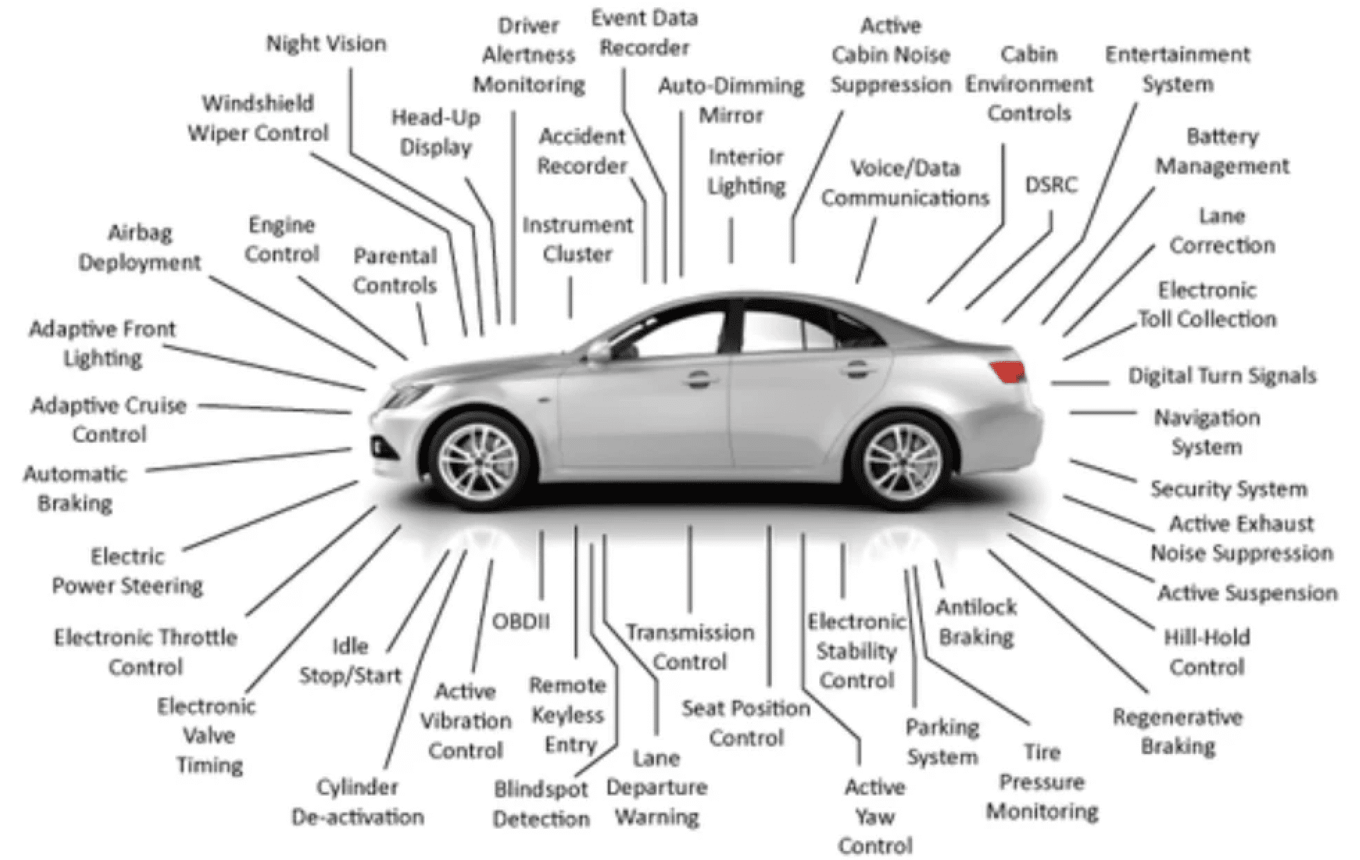
\includegraphics[width=0.9\textwidth]{images/vehicle_processors.png}  % Sostituisci 'nome_immagine' con il nome del tuo file immagine e l'estensione
  \caption{An incomplete overview of computers in a modern car \cite{ieeeSoftwareDefinedVehicle}}
  \label{fig:VheicleProcessors}
\end{figure}

This paradigm shift has been driven in part by the introduction of autonomous driving. To ensure maximum safety, a car must be equipped with dozens of sensors that can constantly collect data about what is happening to the vehicle and its surroundings. The number of these telemetry devices, which are nothing more than specialized IoT devices for the automotive world, also known as \gls{ac:tcu}, is expected to grow as autonomous driving technologies advance. In addition to data collection, another key issue is data analysis. Modern vehicles are caught between low-power systems for maximum vehicle efficiency and high-performance systems for analyzing the collected data and making excellent decisions in a short time.

However, the proliferation of processors within vehicles, orchestrating communication to manage diverse components, presents a formidable challenge; each component often integrates a processor with unique logics, diverging from the logics embedded in processors of other components. Complicating matters further, these components are frequently supplied by companies with proprietary management logics, not readily accessible to the automotive companies themselves.

In addressing this intricate scenario, the transformative concept of a \gls{ac:sdv} comes to the forefront. Defined as "any vehicle that manages its operations, adds functionality, and enables new features primarily or entirely through software"  \cite{blackberrySDV}, the notion of \gls{ac:sdv}, with all the associated technologies, offers a comprehensive solution to the challenges posed by the intricate interplay of software and hardware in modern vehicles.

One of the main benefits of this innovation in the automotive industry is the ability to have easily manageable systems. In the past, due to their high level of specialization for performance and low power consumption, automotive computer systems were developed and tested directly on the devices themselves, often in a manual way. This resulted in a large consumption of resources and a waste of time. Today, the goal is to have cloud infrastructures that ensure a more agile development and testing process due to the presence of general-purpose systems in the vehicle.

Consequently, the use of \gls{ac:sdv} aims to completely separate software and hardware, allowing the production of high-level software on entirely generalized hardware systems. This results in significant savings in terms of time and money for hardware production, along with providing an advantage in terms of security due to the simplification of software.

Another very important aspect of \gls{ac:sdv}, which will be analyzed in the following chapters, is that since a \gls{ac:sdv} is by definition characterized by the ability to dynamically and flexibly update software, this solution offers significant security advantages in several aspects:
\begin{enumerate}
  \item \textbf{Human Safety Critical Security:} From the moment that a vehicle can be classified as safety critical (as it is reported in the standard ISO 26262-1:2018 of the ISO society where is said that "safety is one of the key issues in the development of road vehicles" \cite{ISO26262}), the elimination of software vulnerabilities related to the vehicle's systems is crucial for the overall safety of the vehicle itself.  
  \item \textbf{Intrinsic Software Security:} This approach allows for the prevention and resolution of vulnerabilities unknown at the time of software design, contributing to ensuring a high standard of security. For example, as demonstrated by NIST in the research on the Analysis Of The Impact Of Software Complexity \cite{NISTCodeComplexity}, the increase in software complexity in different cases results in less analyzable programs. In some instances, the same vulnerability analysis tool may detect vulnerabilities, while in others, analyzing the same code, it may not. 
\end{enumerate}

Effectively navigating the development of \gls{ac:sdv} technology necessitates a collaborative approach across diverse companies, particularly in the realms of hardware and cloud computing. For this reason, many software, hardware, and automotive companies are involved in the development of this innovation, which aims to become a standard in vehicle production for the entire automotive industry.

In order to carry out the research and analysis of the new technologies described above, as well as to get involved in the practical side of things, it was essential to find a company that had both the IT skills needed to interface with cloud technologies and experience in the world of automotive manufacturing and software production. The partner company with which the practical design and implementation of the working explanatory example was carried out is introduced below.
\section{Partner Company}

Leveraging extensive experience in the cloud industry and fostering deep-rooted relationships within the automotive sector, Storm Reply stands out as the ideal choice to lead the project discussed in this thesis. A key player in the Reply group, Storm Reply specializes in designing and implementing innovative Cloud-based solutions and services \cite{StormReplySite}. 

With a broad client base spanning multiple sectors, particularly the automotive industry, the company's expertise played a pivotal role in fully understanding the project's context and internal dynamics. This extensive knowledge provided the cornerstone for the development of a tangible example of the infrastructure.

\begin{figure}[h]  % 'h' significa che la figura viene posizionata qui
  \centering
  
\includegraphics[width=0.3\textwidth]{images/Storm_Reply_logo.png}  % Sostituisci 'nome_immagine' con il nome del tuo file immagine e l'estensione
  \caption{Logo of the partenr company of the project}
  \label{fig:StormReplyLogo}
\end{figure}

Among the main customers in the automotive world of the consulting company, we can mention Ferrari, one of the most important companies in motor sports competitions and in the production of luxury cars, and Stellantis, one of the biggest giants in the automotive industry as well as in the global market. Although different, these two companies interact with Storm Reply to take advantage of its great knowledge in the cloud world and in the management of AWS services. Thanks to the connection with these important companies it was possible to receive essential information for the thesis work.

One great advantage of collaborating with this company is the wide availability of resources, both material and, above all, in terms of experience. As a large IT consultancy company, Reply is divided into many sub-business units, that makes possible the nteraction with various realities, ranging from embedded to low-level development, network and security infrastructure management, and web services management. Furthermore, there is a research and development section called Area 42 where entities can interact and influence each other to create innovative projects.

A point of pride for Storm Reply is its recognition as an Amazon Web Services (AWS) Premier Consulting Partner since 2014, ranking among the top Amazon Partners globally. This distinctive characteristic underscores the decision to develop the infrastructure using Amazon Web Services.

According to the official AWS description page \cite{AWSGlobalInfrastructure} the AWS Cloud spans 102 Availability Zones within 32 geographic Regions around the world and servs 245 countries and territories. With millions of active customers and tens of thousands of partners globally, AWS has the largest and most dynamic ecosystem. AWS is evaluated as a Leader in the 2022 Gartner Magic Quadrant for Cloud Infrastructure and Platform Services (a series of market research reports published by IT consulting firm Gartner that rely on proprietary qualitative data analysis methods to demonstrate market trends, such as direction, maturity and participants), placed highest in Ability to Execute axis of measurement among the top 8 vendors named in the report.

\begin{figure}[h]  % 'h' significa che la figura viene posizionata qui
  \centering
  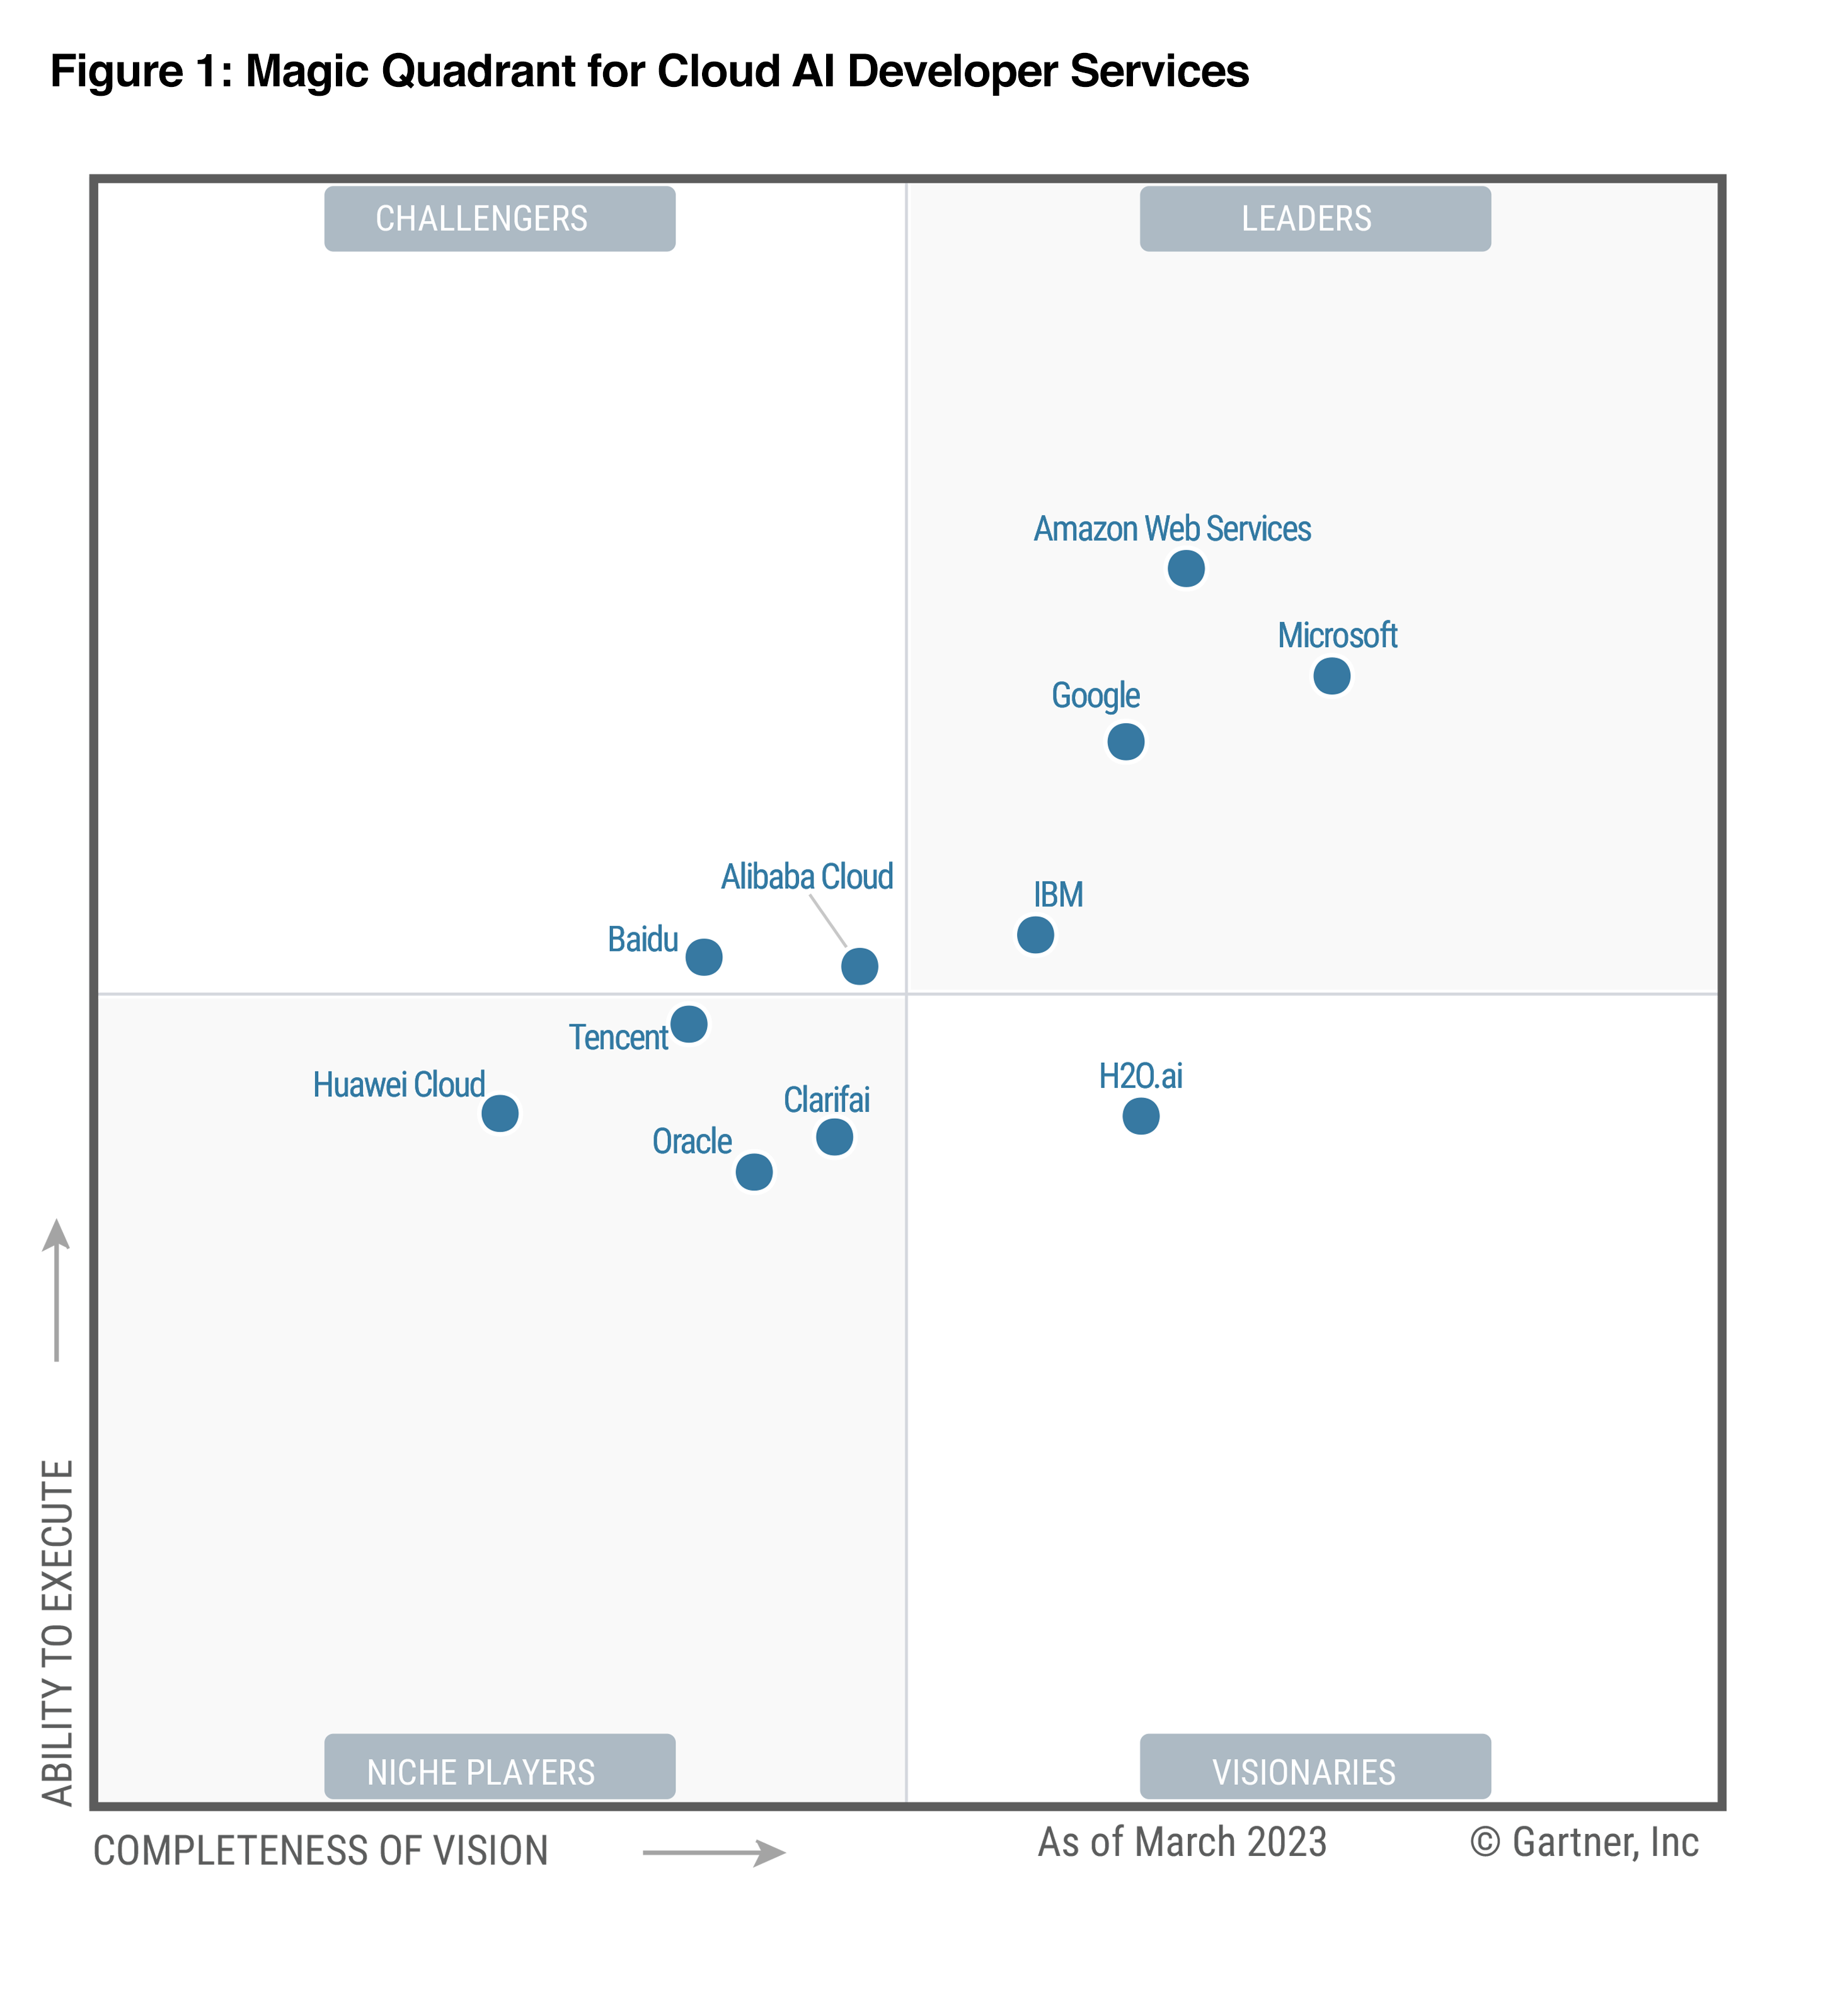
\includegraphics[width=0.6\textwidth]{images/AWSMagicQuadrantForCloud.png}  % Sostituisci 'nome_immagine' con il nome del tuo file immagine e l'estensione
  \caption{The Gartner Magic Quadrant for Cloud Infrastructure and Platform Services \cite{GartnerMagicQuadrant}}
  \label{fig:AWSMagicQuadrantForCloud}
\end{figure}

The infrastructure exhibits several key attributes contributing to its robustness and efficiency: 
\begin{itemize} 
  \item \textbf{Security:} The infrastructure undergoes 24/7 monitoring to ensure the confidentiality, integrity, and availability of data. All data flowing across the AWS global network is automatically encrypted at the physical layer before leaving secured facilities.
  \item \textbf{Availability:} To ensure high availability and isolate potential issues, applications can be partitioned across multiple AZs (Availability Zones) within the same region, creating fully isolated infrastructure partitions.
  \item \textbf{Performance:} AWS Regions offer low latency, low packet loss, and high overall network quality. This is achieved through a fully redundant 100 GbE fiber network backbone, often providing terabits of capacity between Regions.
  \item \textbf{Scalability:} The AWS Global Infrastructure allows companies to take advantage of the virtually infinite scalability of the cloud. This enables customers to provision resources based on actual needs, with the ability to instantly scale up or down according to business requirements.
  \item \textbf{Flexibility:} The AWS Global Infrastructure provides flexibility in choosing where and how workloads are run, whether globally, with single-digit millisecond latencies, or on-premises.
  \item \textbf{Global Footprint:} AWS boasts the largest global infrastructure footprint, continually expanding at a significant rate.
\end{itemize}
Thanks to its expertise and qualifications, Storm Reply is able to provide the above features to its customers, offering a comprehensive consultancy service for managing cloud infrastructures.

\section{Thesis Objective}
In the automotive context, the use of \gls{ac:sdv} plays a crucial role in terms of cost, innovation and safety. The objectives of the thesis are intertwined with the opportunities offered by \gls{ac:sdv} technology, for instance addressing the primary challenge of overcoming the current difficulties associated with the presence of different specialized hardware platforms on the same vehicle, to make the vehicle a more efficient and safer device based on software as a fundamental element.

One of the main objectives of this thesis is to propose the opportunity offered by \gls{ac:sdv} solution capable of eliminating various phases of the software production pipeline. This would result in significant time and cost savings, enabling the investment of these resources in other areas.

From a practical standpoint, the project's goal is to provide, through the use of AWS services, a cloud infrastructure capable of managing the \gls{ac:sdv} both in terms of software production and data analysis.

The work begins with an overview of the state of the art of software development in the automotive world, comparing the goals of the future with the techniques used in the past. For this purpose, the weaknesses of the sector are explained in order to highlight the advantages of \gls{ac:sdv} technology.Next, some definitions of the technologies that can bring the development of a paradigm shift in \gls{ac:sdv} benefits are provided. Finally, an example of an initiative proposed as a first attempt to standardize the \gls{ac:sdv} concept is presented, namely the SOAFEE project.

The work continues with an introduction to cloud computing, which is the programming approach that accompanied the entire project from beginning to end. The characteristics of this technique are analyzed, especially the advantages it can bring, and the example of how AWS manages to best enhance the potential of cloud computing is shown. Special attention is given to the security aspect, as it is a fundamental objective of the thesis topic, but also central element of the idea behind the cloud development of the AWS company and the project partner company.

Moving towards the description of the implementation of the practical project, it is possible to arrive at the exploration of the AWS services used. In order to make the realization of the project possible, as described several times throughout the thesis, it is necessary to rely on this type of service. With the aim of introducing the characteristics of the services used, an extensive descriptive list is provided.

The last part of the thesis deals with the actual implementation of the project, with the purpose of providing a concrete and working example of what has been described in the previous chapters. The implementation begins with the creation from scratch of a device capable of simulating telematic data, develops in the construction of a cloud infrastructure with the services mentioned above, and ends with the exploration of the tool used for data analysis.

Finally, to conclude the research, the results of the final presentation of the operation of the whole system on a real device are shown. In addition, a final evaluation of the whole project is made and the future possibilities opened by the work are shown.
\lstdefinestyle{mystyle}{
    backgroundcolor=\color{myyellow},
    basicstyle=\ttfamily\small,
    breaklines=true,
    frame=single,
    language=XML
}

\chapter{State-of-the-Art Analysis} \label{ch:state-of-the-ArtAnalysis}
The following chapter constitutes an in-depth exploration of current technologies and methodologies within the automotive industry, with a specific focus on the complexity of vehicular software development. Firstly, the current automotive landscape will be examined, providing a detailed insight into challenges associated with software development in vehicles.

Subsequently, through meticulous analysis of scientific publications, technical reports, and practical implementations, the chapter delves into the radical transformation of the automotive sector facilitated by the concept of Software Defined Vehicle (SDV). This technology, crucial for technological progress and vehicular safety, will be explored from various perspectives. Particularly, the synergy between Cloud, software, and hardware will be investigated, highlighting solutions proposed by major industry players and analyzing their applications, benefits, and limitations.

The objective is to offer a comprehensive overview of current dynamics, emphasizing the pivotal role of SDV in the evolution of the automotive industry.

\section{Current Automotive Software Development}

In the past, the automotive industry advanced primarily through the development of technologies in mechanical engineering, focusing on perfecting combustion engines. Nowadays, the paradigm has radically changed due to multiple factors, including electrification, automation, shared mobility, and connected mobility.

Software technology development in the automotive field can be metaphorically compared to what has happened in smartphone development, as highlighted in the manifesto document regarding Bosch's Software Defined Vehicle (SDV) \cite{SDVBoschMobility}.

The ultimate goal is to achieve simple and user-friendly devices that fully meet the user's needs. Currently, many customers express dissatisfaction because their cars do not offer the same functionality and ease of use common in smartphones. Many ask: Why can't my \$50,000 car perform the same tasks as my \$300 smartphone?

A key difference between the automotive and smartphone industries is the level of complexity, which brings with it a number of issues.

\subsection{difficulties}
We can analyse in depth the problems of the current automotive software that is being developed via 4 main difficulties:

\begin{itemize}
    \item \textbf{Specialized Hardware:} Today's vehicles are still complex systems of systems. Each subsystem in a car, from brakes to transmission, is a complex entity, supplied by a different manufacturer and integrated with a unique software architecture. The level of complexity and the need for seamless interoperability between systems far exceeds that of today's smartphones.
    \item \textbf{Time:} The software production pipeline involves many development and testing steps with a not inconsiderable amount of time spent on each one. This is greatly increased by the presence of different components, so development time must be considered for each different unit of the system.
    \item \textbf{Cost:} The complexity of the software systems in vehicles entails very high costs, aggravated by the fact that the test phase is often carried out directly on the boards (for hardware requirements), which means a much longer production process, especially in the event of errors.
    
    \begin{figure}[h]  % 'h' significa che la figura viene posizionata qui
        \centering
        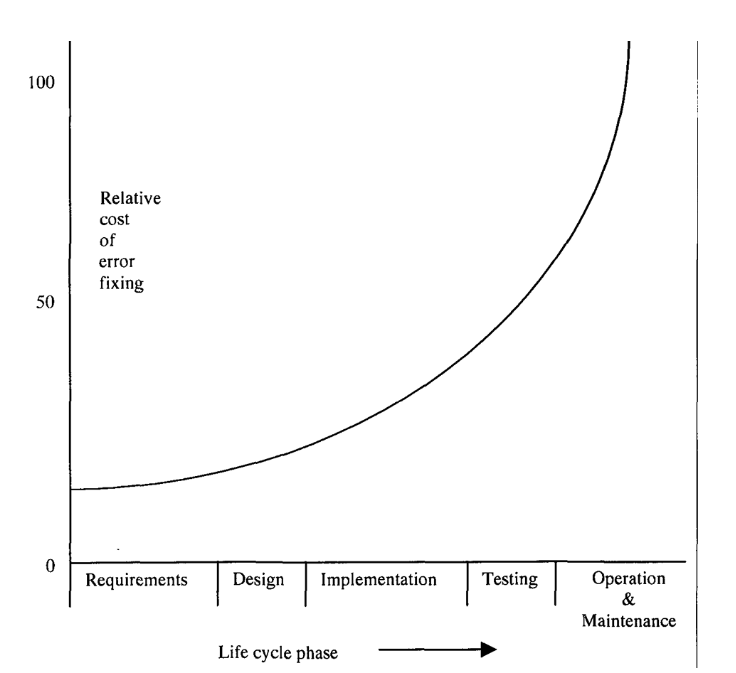
\includegraphics[width=0.9\textwidth]{images/costs_of_errors_correction_in_software_development.png}  % Sostituisci 'nome_immagine' con il nome del tuo file immagine e l'estensione
        \caption{Cost of fixing errors increases in later phases of the life cycle \cite{CostsOfSoftwareDeveloping}}
        \label{fig:CostsOfSoftwareDeveloping}
      \end{figure}

    \item \textbf{Human Safety Security:} Automotive embedded software must meet stringent reliability and security requirements, while delivering performance and a reasonable memory footprint. To develop automotive embedded software, you need the right tools that meet safety and security standards to evaluate, prototype and test your software.
\end{itemize}

What lessons can be drawn from the study of barriers that can be applied to the vehicle lifecycle? Historically, the vehicle lifecycle has been characterised by the simultaneous production and deployment of tightly integrated hardware and software. Once the vehicle was in the hands of the consumer, its characteristics remained largely unchanged until the end of its life. However, the SDV paradigm introduces the possibility of decoupling hardware and software release dates, a prerequisite for adopting a digital-first approach. This approach brings the design and virtual validation of the digital vehicle experience to the forefront of the lifecycle.
It also requires the application of the digital-first concept, which means that new ideas for the vehicle experience are first explored in virtual environments to ensure early user feedback, long before any custom hardware needs to be developed or a physical test vehicle is available. Digital first is the application of design thinking and lean startup principles, originally rooted in internet culture, to the tangible realm of automotive development.

%“Automakers and their suppliers need to continuously review and improve the testing approach in design and development, as well as look for new tools that automate and increase test coverage of their products,” Giallorenzo explained. “Cloud emulation is a major innovation that is coming to the industry to facilitate development and testing. Historically, testing of embedded software solutions has been hindered by the lack of chipsets and hardware, which is required to properly test complete hardware-plus-software solutions. This was particularly painful during the recent COVID-induced supply chain crunch."

\section{Introduction to Software Defined Vehicle}
The Software Defined Vehicle represents the new frontier of automotive manufacturing and is poised to completely change the paradigm of automotive production. 

If we imagine bringing a feature update to one of today's vehicles, it will most likely take anywhere from one to seven years from the idea to when that feature is actually perceptible in the production vehicle; this takes so long because the vehicles produced up to this point have not been designed with frequent updates in mind \cite{SDVBosch}.
Traditionally focused on physical functionality, the automotive industry has evolved from early electronic features such as airbags, vehicle stabilisation and braking systems to modern driver assistance and even automated driving. 
The current shift towards a digital experience is possible thanks to vehicle design that includes software integration as a fundamental part. Software should no longer be seen as an accessory to the vehicle, but as an integral part of the vehicle itself.

The simultaneous efforts of major automotive companies such as Bosch, Renault and Stellantis, in collaboration with leading computer developers such as Arm, BlackBerry and AWS, have given rise to the Software Defined Vehicle concept, which they define as "any vehicle that manages its own operations, adds functionality and enables new features primarily or entirely through software" \cite{blackberrySDV}.

The Software Defined Vehicle solution is nowadays being considered by several companies as the manifesto of a new era of vehicle development. An example is given by the Renault Group, which in an overview of its products describes: "Today, it is already possible to make remote updates of some vehicles via the Firmware Over The Air (FOTA) system. This keeps the vehicle safe by making it easier and faster to improve the on-board system and apply patches. Tomorrow, the Software Defined Vehicle's flexible and scalable architecture will enable the faster development and integration of new features throughout the vehicle lifecycle, directly into the cloud, that is, in secure online servers accessible from anywhere and anytime" \cite{SDVRenault}. 

It is evident that Software Defined Vehicles represent the future of the automotive industry, promising an enriched and sustainable user experience as vehicle technologies evolve. This section further clarifies the current state of the industry, highlighting the key enablers that are allowing the development of the SDV paradigm and the benefits of this innovation.

\subsection{Enablers}

There are mainly three fundamental technologies that contribute to the realisation of the Software Defined Vehicle: standardized hardware, cloud and over-the-air (OTA) updates via OTA servers, all developed by leading companies in the computing industry. In this section, each technology will be analysed with reference to concrete examples from the current market.

\begin{itemize}
    \item \textbf{Standardized hardware} 
    
    One of the most important aspects of Software Defined Vehicle is the separation of software from hardware. To achieve this, it is essential to move away from the approach of using dedicated hardware for each vehicle component system, and instead favour an approach based on general purpose processors that are as centralised as possible. This transition not only promotes ease of software development and scalability, but also offers the opportunity to create parity between the virtual development and test environment and the real execution environment.
    
    Several players in the semiconductor industry have stepped up to the challenge of realising this vision, including Arm. Through the development of energy-efficient processors, Arm is present in every part of the vehicle, from high-performance systems in advanced driver assistance systems (ADAS), automated driving (AD), in-vehicle infotainment (IVI) and digital cockpits, to gateway, body and microcontroller endpoints \cite{ArmAutomotive}. The aim is to create Arm-based MCUs that enable implementation of a common architecture, scalability between applications to meet processing requirements, software reuse and reduced development costs.
    
    Another major player is Qualcomm, which is being adopted by the Renault Group through its Snapdragon Digital Chassis vehicle architecture, a set of cloud-connected platforms for telematics and connectivity, digital cockpits, assistance and driver autonomy.

    \item \textbf{Cloud} 
    
    Using a cloud platform that offers scalable and secure solutions for real-time application updates, increased connectivity and efficient data management is essential for SDV. 

    Well-known companies such as Amazon Web Services (AWS) and Google Cloud are already present in the automotive industry as partners of partner of many automotive companies. The AWS services and technologies will be in depth described in the futher chapters.
 
    \item \textbf{Over-The-Air updates}
    
    An Over-The-Air (OTA) update is the remote and wireless transfer of applications, services, firmware and configurations from a server to a target device. This process takes place over an available network, preferably the Internet. The main purposes of OTA are to remotely update software or firmware, provide power-safe procedures to ensure that the device will boot even if power is lost during the update process, maintain a robust implementation, ensure data protection and reduce overall maintenance costs \cite{Open-sourceSWUpdate}.

    In the context of the thesis, it is crucial to acknowledge that the implementation of OTA updates may increase the vulnerability of automotive systems to hacking and other cyber attacks. These vulnerabilities could potentially be exploited by hackers to gain unauthorised access to private information, take remote control of the vehicle or even cause it to malfunction. Another significant issue is the leakage of information about updates and their sources. This can enable malicious actors to introduce viruses and malware, further exacerbating the security risks associated with OTA updates \cite{EnhancedMulti-LevelSecureUpdate}. 
    
    To perform an OTA update, both a client on the vehicle, responsible for waiting and checking for incoming updates, and a server, facilitating the availability of the update broadcast to all connected devices, are essential. In this context, Autosar can be considered, as it represents a standard and open source architecture for intelligent mobility \cite{AutosarAbout}, which includes a dedicated platform for client and server management of OTA updates. Another notable example is Hawkbit, which serves as a backend framework for deploying software updates to edge devices and is being developed by the Eclipse Foundation; this tool will be discussed in more detail in later chapters as it will be used to create a proof of concept. The final tool of note is AWS Greengrass, an edge agent manager for managing software updates in edge IoT devices, provided by AWS; this tool will also be discussed in later chapters as an alternative solution to the client manager.
    
    \item \textbf{MQTT communication}
    
    The Message Queuing Telemetry Transport (MQTT) is a standardized protocol, specified by ISO/IEC 20922:2016 and developed by the Oaesis organization. It enables the exchange of Application Messages over a network connection, providing an ordered, lossless stream of bytes from the Client to Server and Server to Client without the need to support of a specific transport protocol.

    In an MQTT transport, an Application Message carries payload data, a Quality of Service (QoS), a collection of Properties, and a Topic Name. Clients, which can be programs or devices, perform various actions such as opening and closing network connections, publishing Application Messages, subscribing to requested Application Messages, and managing subscriptions \cite{MQTTVersion5.0}.

    On the Server side, it acts as an intermediary between publishing and subscribing Clients. The Server accepts network connections, processes Subscribe and Unsubscribe requests, and forwards Application Messages matching Client Subscriptions. The Server, also known as the Broker, essentially coordinates messages among various Clients. Its responsibilities extend to authorizing and authenticating MQTT Clients, transmitting messages to other systems for further analysis, and managing tasks such as handling missed messages and Client sessions \cite{MQTTAWS}.

    Sessions, representing stateful interactions between Clients and Servers, can last for the duration of a Network Connection or span multiple consecutive connections.
     \begin{figure}[h]  % 'h' significa che la figura viene posizionata qui
        \centering
        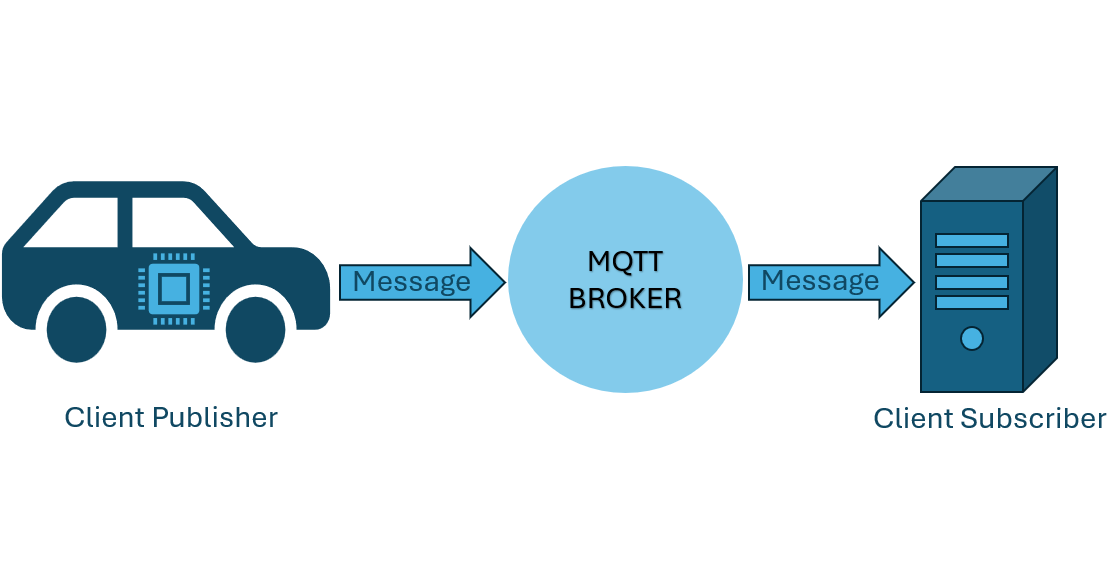
\includegraphics[width=0.8\textwidth]{images/MQTTProtocol.png}  % Sostituisci 'nome_immagine' con il nome del tuo file immagine e l'estensione
        \caption{A simple representation of communication using the MQTT protocol}
        \label{fig:MQTTProtocol}
    \end{figure}

    The MQTT protocol can be used in SDV, both for sending data produced by the vehicle to the cloud servers and for sending updates from the servers to the vehicle. This is because the MQTT protocol allows asynchronous and misaligned communication even in the presence of poor connectivity, a situation that cannot be underestimated in the automotive field.
\end{itemize}

The collaborative efforts of this technologies contribute to advancement of SDV for makeing vehicles not only defined by their physical attributes but also as dynamic entities that can be continuously updated through software.

\subsection{Benefits}
The Software Defined Vehicle, as introduced in the previous chapters, brings several benefits to both automotive companies and the end-user experience.  These innovations are made possible by the fact that the vehicle becomes a device that can be constantly monitored and updated in real time via the cloud throughout its entire lifecycle. Let us now look at the key benefits.

From the point of view of this project, the main innovation brought by this technology is the security of the device software. Since, as mentioned above \cite{ISO26262}, vehicles are considered as safety elements critical to human life, the safety benefits can be analysed from two perspectives:
\begin{itemize}
    \item \textbf{Human Safety Critical Security:} The ability of SDV to receive real-time data from the vehicle allows in-depth monitoring of all its components. Taking the influence of tyres as an example, it has been found that most road accidents are caused by tyre wear and lack of regular maintenance. It is therefore necessary to assess the health of tyres through continuous monitoring of physical parameters such as tyre thickness, temperature and pressure, as well as regular maintenance. This helps to eliminate or minimise the possibility of tyre bursts and subsequent accidents. It also improves the safety of people and vehicles \cite{PredictDefectsOfTiresInHeavyVehicle}. These factors can be monitored either manually or automatically: manual predictive maintenance requires human intervention and can lead to some errors; automatic predictive maintenance using artificial intelligence can be more efficient \cite{AirPressureSystemFailurePrediction}. Renault defines this work as "predictive maintenance" \cite{SDVRenault}, stressing the importance of collecting and analysing data in a centralised system to anticipate and prevent potential failures, ensure the safety of people, reduce maintenance costs and improve the performance of the vehicle.
    \item \textbf{Intrinsic Software Security:} In the presence of bugs and vulnerabilities in the vehicle's software, SDV makes it possible to intervene promptly to resolve each problem and reduce the window of exposure.
    \begin{figure}[h]  % 'h' significa che la figura viene posizionata qui
        \centering
        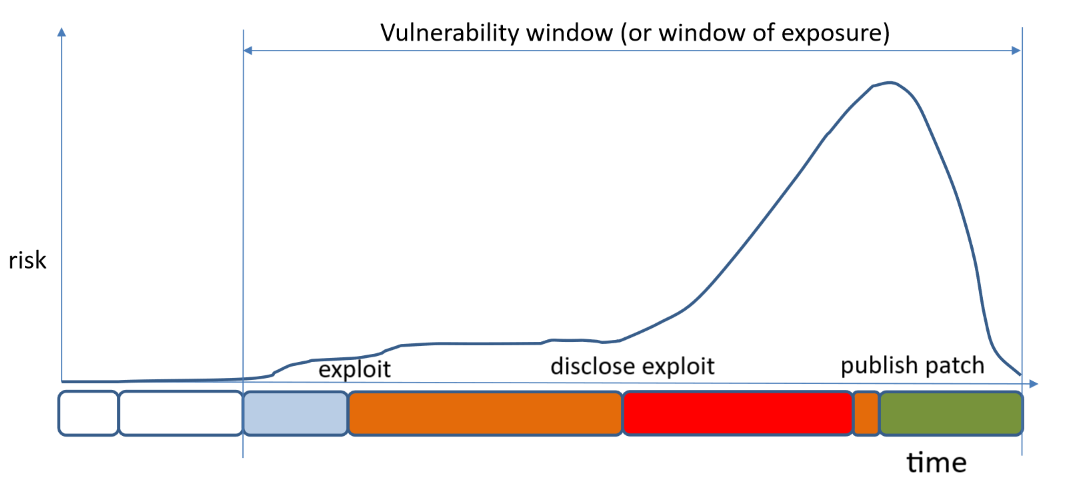
\includegraphics[width=0.8\textwidth]{images/window_of_exposure.png}  % Sostituisci 'nome_immagine' con il nome del tuo file immagine e l'estensione
        \caption{Risks and time relationship in the various phases of a vulnerability lifecycle}
        \label{fig:WindowOfExposure}
    \end{figure}

    A crucial aspect of vehicle software security is the robustness of the algorithms, especially in the context of autonomous driving. In this context, a predictive algorithm responsible for vehicle safety decisions can be continuously improved and optimised. The SDV also introduces the concept of the 'digital twin', a platform that virtually replicates the functionality and behaviour of the vehicle. Thanks to this technology, predictive algorithms used in autonomous driving can be effectively tested on the cloud platform and, when ready, integrated directly into the vehicle.
\end{itemize}

From a user experience point of view, two other significant benefits can be identified: an increase in the value of the vehicle, which can be continuously upgraded over time, and the ability to enable additional vehicle functions via software. For example, the user can decide to activate a feature for a certain period of time and then deactivate it (paying only for the time it is used), or activate a new feature that was not available at the time of purchase. In essence, the vehicle becomes a dynamic platform that is constantly evolving and fully customisable through the software.

For automotive companies, the benefits mentioned so far can bring direct benefits to the industry. In support of this, Stellantis reports that: "the team in Poland will contribute to the global software creation network that is key to Stellantis' work in creating software-defined vehicles (SDVs) that offer customer-focused features throughout the vehicle's life span, including updates and features that will be added years after the vehicle is manufactured. “Creating an infrastructure inside our vehicles that easily and seamlessly adapts to meet driver expectations is a key element of Stellantis' global drive to deliver cutting edge mobility. Stellantis' software-driven strategy deploys next-generation tech platforms, building on existing connected vehicle capabilities to transform how customers interact with their vehicles and to generate €20 billion in incremental annual revenues by 2030".

In addition, the SDV paradigm brings an advantage from a software production pipeline perspective. In today's software production scenario, there can be two development mechanisms:
\begin{itemize}
    \item A more traditional mode in which software is created directly on the system, hence on the processor itself. This is undoubtedly the most inconvenient solution, as it would require unnecessary overuse of processors, wasting resources, money and time.
    \item Alternatively, developers rely on cumbersome operating system emulation tools on the host machine and the cross-compilation process, which uses a dedicated compiler to produce executable code for the target system. Once the code is on the development system, a final integration and validation test can be performed, but scalability is limited to the number of physical hardware platforms. 
\end{itemize}

Typical workflows for the development, integration and validation of embedded systems are as follows \cite{DevelopersWorkflow}:
\begin{figure}[h]  % 'h' significa che la figura viene posizionata qui
    \centering
    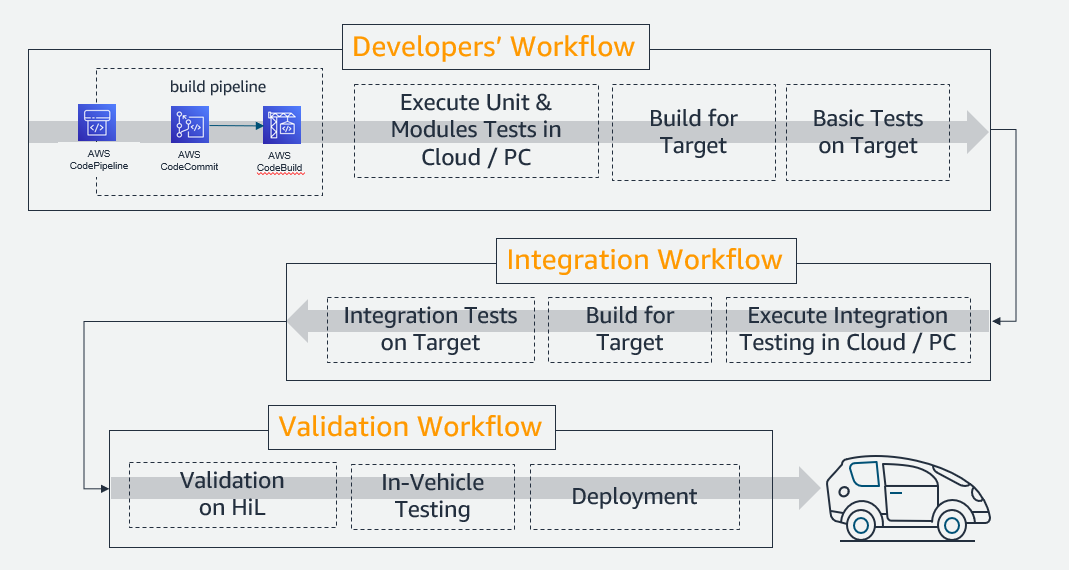
\includegraphics[width=0.7\textwidth]{images/today_developer_workflow.png}  % Sostituisci 'nome_immagine' con il nome del tuo file immagine e l'estensione
    \caption{today development, integration, and validation workflows for embedded systems}
    \label{fig:TodayDeveloperWorkflow}
\end{figure}

As explained in the following chapters, by using the software defined vehicle, i.e. operating systems that rely on general purpose porpouse architectures to provide parity between cloud and edge systems, it is possible to reduce the embedded developer's workflow to remove many of the steps that are now no longer required, as shown in the diagram below \cite{DevelopersWorkflow}:
\begin{figure}[h]  % 'h' significa che la figura viene posizionata qui
    \centering
    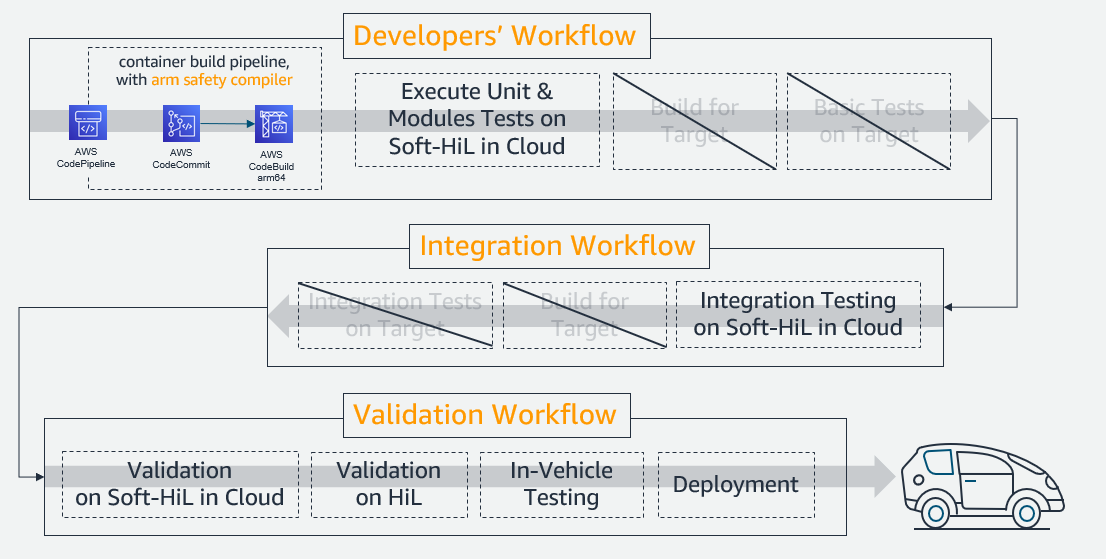
\includegraphics[width=0.7\textwidth]{images/future_developers_workflow.png}  % Sostituisci 'nome_immagine' con il nome del tuo file immagine e l'estensione
    \caption{future development, integration, and validation workflows for embedded systems}
    \label{fig:FutureDevelopersWorkflow}
\end{figure}

\subsection{initiatives: SOAFEE}
In 2021 Arm, AWS, and other founding members announced the Scalable Open Architecture for Embedded Edge (SOAFEE) Special Interest Group, which brings together automakers, semiconductor, and cloud technology leaders to define a new open-standards based architecture to implement the lowest levels of a software-defined vehicle stack. \cite{DevelopersWorkflow}

SOAFE is created to achive Software Defined Vehicle, and for doing that four-pillar principle are used \cite{SoafeeProject}:
\begin{enumerate}
    \item Standards: standardization ensures interoperability and compatibility among various software components, fostering a cohesive ecosystem for Software Defined Vehicles.
    \item New software architecture and methodologies: this involves transitioning from traditional monolithic architectures to more modular and scalable designs; the incorporation of agile development practices and DevOps methodologies ensures efficient and continuous software evolution.
    \item Industry collaboration: Fostering partnerships, knowledge sharing and collaboration among key stakeholders, including automakers, technology companies and regulators, is essential.
    \item Vehicle simulation: simulated environments allow in-depth testing and refinement of software functionality to ensure optimal performance and security under a variety of conditions.
\end{enumerate}
SOAFEE aims to adopt and enhance current standards used in today's cloud-native world to help manage the software and hardware complexity of the automotive Software Defined Vehicle architecture.

The core principles of safety, security, and real time are inherent in each pillar. It is fully expected that the SOAFEE architecture will support use-cases that execute safety-critical services alongside non-safety-critical ones. It is fully expected that the SOAFEE architecture will support use cases that execute safety-critical services alongside non-safety-critical services. As it is not reasonable to develop the whole platform according to one safety standard, the strategy is to develop only safety-critical elements according to ISO 26262 and to isolate them from the non-safety-critical elements in order to ensure spatial, temporal and communication isolation. All implementations pass security checks and follow a set of best practices /cite{SoafeeArchitectureOverview}.

The SOAFEE paradigm is based on a very sophisticated architecture becouse it should work in the same way in the vehicle and in the cloud and follow cloud native technologies while considering the automotive specific needs for safety and limited resource footprints \cite{SoafeeArchitecture}.
\begin{figure}[h]  % 'h' significa che la figura viene posizionata qui
    \centering
    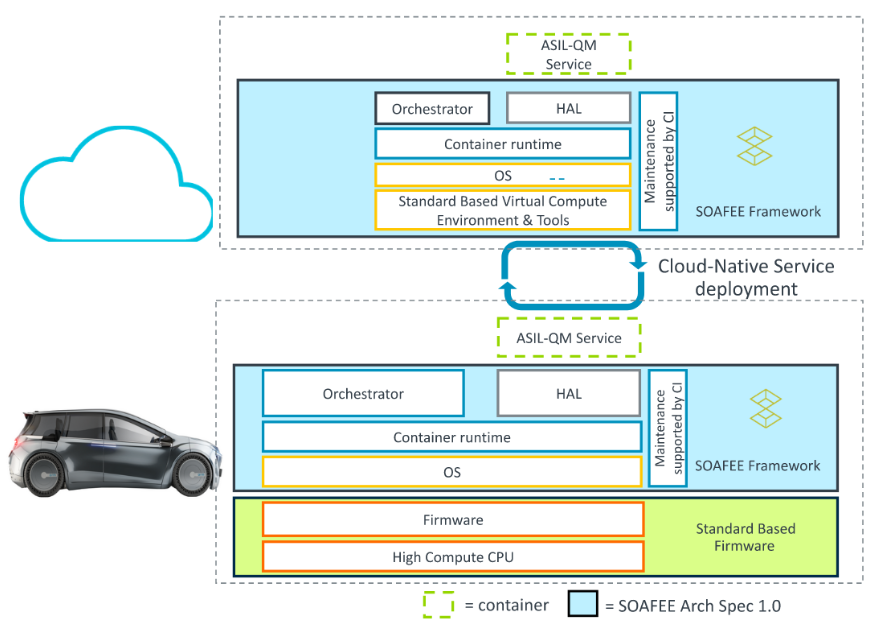
\includegraphics[width=0.7\textwidth]{images/SOAFEE_architecture.png}  % Sostituisci 'nome_immagine' con il nome del tuo file immagine e l'estensione
    \caption{SOAFEE Architecture v1.0 \cite{SoafeeArchitecture}}
    \label{fig:SoafeeArchitecture}
\end{figure}
\lstdefinestyle{yaml}{
     basicstyle=\color{red}\footnotesize,
     rulecolor=\color{black},
     string=[s]{'}{'},
     stringstyle=\color{red},
     comment=[l]{:},
     commentstyle=\color{black},
     morecomment=[l]{-}
 }
 
\chapter{Cloud Computing and Amazon Web Services} \label{ch:CloudComputingAndAmazonWebServices}

As the analysis in previous chapters has shown, the \gls{ac:sdv} is a pivotal advancement in the evolution of the entire automotive industry toward a safer, more efficient, and more sustainable future. Cloud computing is a crucial resource for \gls{ac:sdv} development due to its facilitation of development through its features and benefits. In the following section, cloud computing technologies will be analyzed in detail, focusing on one of the most important providers, \gls{ac:aws}.
\section{Cloud Computing}
The National Institute of Standards and Technology (NIST) provides the most comprehensive definition of cloud computing: "Cloud computing is a model for enabling ubiquitous, convenient, on-demand network access to a shared pool of configurable computing resources (e.g., networks, servers, storage, applications, and services) that can be rapidly provisioned and released with minimal management effort or service provider interaction. This cloud model is composed of five essential characteristics, three service models, and four deployment models" \cite{NISTCloudComputing}. This allows for a thorough analysis of the features of cloud computing in relation to \gls{ac:aws} services, starting with the five essential characteristics.
\begin{itemize}
    \item \textbf{On-demand self-service:} Consumers can access and allocate computing resources autonomously, such as server time and network storage, without direct involvement with service providers. \gls{ac:aws} offers a vast cloud infrastructure with over 200 fully-featured services that consumers can easily access and use from their \gls{ac:aws} account.
    \item \textbf{Broad network access:} Resources can be accessed over the network through standard mechanisms, making them usable across various client platforms. In \gls{ac:aws} services, this is translated as an on-demand delivery of IT resources over the Internet with pay-as-you-go pricing. 
    \item \textbf{Resource pooling:} Providers pool computing resources in a multi-tenant model, dynamically assigning them based on consumer demand. As said before \gls{ac:aws} services are allocable e pagabili in base alle necessità del momento. The customer has limited control over the exact resource location but can specify a higher-level abstraction as country, state, or datacenter. In \gls{ac:aws}, clients can select the geographic location of their services through regions. \gls{ac:aws} Regions provide access to \gls{ac:aws} services that are physically located in a specific geographic area. \gls{ac:aws} provides the option to view the availability of a particular service in a specific region, in addition to selecting different regions \cite{AWSRegions}. Resources include storage, processing, memory, and network bandwidth. It also provides services for the Internet of Things, machine learning, data lakes, and analytics.
    \item \textbf{Rapid elasticity:} Resources can be easily adjusted to match fluctuations in demand, either automatically or manually. \gls{ac:aws} provides various automated resource allocation systems, including the \gls{ac:aws} Cloud Development Kit (\gls{ac:aws} CDK) framework, which will be discussed later. The available capabilities are perceived as virtually limitless, and consumers can acquire them in any quantity at any time, always with a pay-per-use system.
    \item \textbf{Measured service:} Cloud systems efficiently manage resources through automated control and optimization, utilizing metering capabilities tailored to specific services such as storage, processing, bandwidth, and user accounts. For instance, \gls{ac:aws} has infrastructure worldwide, allowing for easy deployment of applications in multiple physical locations. The proximity to end-users reduces latency and enhances their experience. This feature allows for clear and objective monitoring, control, and reporting of resource usage by both providers and consumers.
\end{itemize}

The three primary types of cloud computing are Infrastructure as a Service (IaaS), Platform as a Service (PaaS), and Software as a Service (SaaS). These options provide different levels of control, flexibility, and management, allowing users to configure services to meet their specific requirements.
\begin{itemize}
    \item \textbf{Infrastructure as a Service (IaaS): } Consumers are able to utilize and deploy fundamental computing resources, including processing, storage, and networks. However, they only have control over operating systems, storage, and applications, as the cloud infrastructure is managed by the provider. Consumer control over some networking components is limited. Infrastructure as a Service (IaaS) provides a high level of flexibility and management control over IT resources. It is similar in practice to existing IT resources that many IT departments and developers are already familiar with. 
    \item \textbf{Platform as a Service (PaaS): } Consumers can deploy their applications on the cloud infrastructure using the programming languages, libraries, services, and tools supported by the provider. The provider manages the underlying cloud infrastructure, including network, servers, operating systems, and storage, while consumers maintain control over their applications and configuration settings. This approach improves efficiency by eliminating the need to manage resource procurement, capacity allocation, software maintenance, patching, or any other tasks involved in running your application. 
    \item \textbf{Software as a Service (SaaS): } Consumers can use the provider's applications on the cloud infrastructure, which are accessible from different client devices through interfaces such as web browsers or programs. However, consumers do not have control over the underlying cloud infrastructure, including the network, servers, operating systems, and storage, except for limited user-specific application configuration settings. With a SaaS offering, users do not need to worry about maintaining the service or managing the underlying infrastructure. The focus should be on how to use the software effectively.
\end{itemize}

The analysis thus far has focused on cloud computing, specifically the essential characteristics that a cloud service must possess to be considered a true cloud service, as well as the service models that can be offered. Now, let's analyze in more detail the part related to cloud computing service deployment models and explore which models are most suitable for which workloads using \gls{ac:aws} \cite{AWSPrivatePublicHybrid}. Note that in this case, there are slight differences between the NIST and \gls{ac:aws} definitions of the various deployment modes.
\begin{itemize}
    \item \textbf{public cloud: } According to NIST, a public cloud is defined as cloud infrastructure that is publicly accessible and owned, managed, and operated by businesses, academic institutions, government entities, or a combination thereof. In contrast, \gls{ac:aws} defines a public cloud as infrastructure and services that are accessible over the public internet and hosted in a specific \gls{ac:aws} Region.
    \item \textbf{private cloud: } Both NIST and \gls{ac:aws} define private cloud as a cloud infrastructure exclusively provisioned for a single organization, which may own, manage, and operate it independently or in collaboration with a third party. However, there is a difference in the location of the infrastructure. According to NIST, the infrastructure can be located on or off premises, while in \gls{ac:aws} documentation, the infrastructure is provisioned on premises using a virtualization layer.
    \item \textbf{hybrid cloud: } The hybrid cloud is a combination of two or more separate cloud infrastructures, private or public, connected by technology to facilitate data and application portability. It allows organizations to leverage the cloud for its efficiency and cost savings while also maintaining on-site security, privacy, and control.
\end{itemize}

Exploring the many benefits of cloud computing, the focus now shifts to a comprehensive analysis of the main value patterns of cloud computing, with some charts and graphs to help clarify the outlook.

\begin{table}[h]
    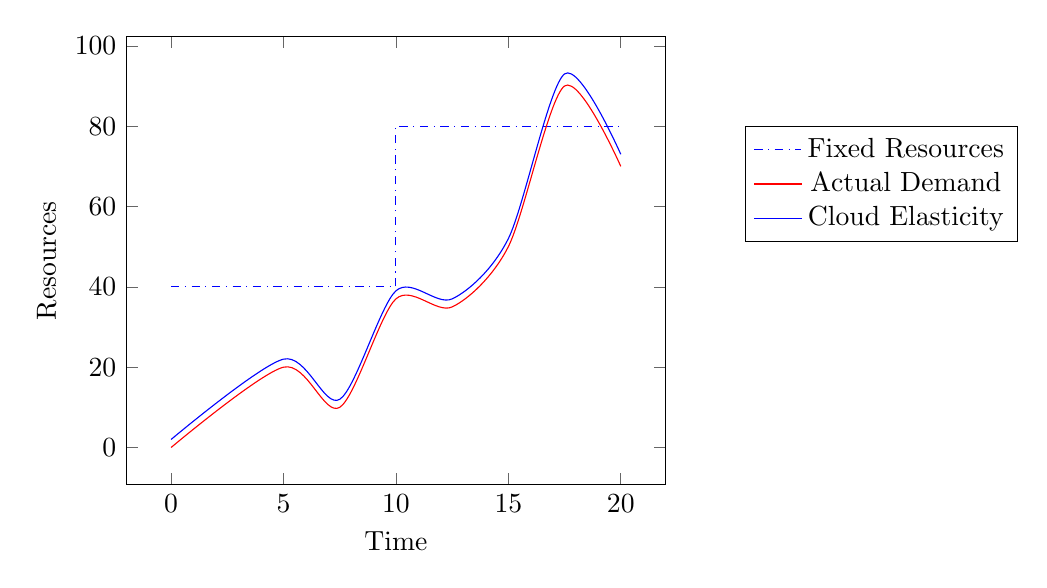
\begin{tikzpicture}
        \begin{axis}[xlabel={Time}, ylabel={Resources}, legend style={at={(1.4,0.8)},anchor=north},]
            % Fixed Resources line
            \addplot[blue,mark=none, dash dot] coordinates {(0,40) (10,40) (10,80) (20,80)};
            \addlegendentry{Fixed Resources}
        
            % Actual Demand line
            \addplot[red,mark=none, smooth] coordinates {(0,0) (5,20) (7.5,10) (10,37) (12.5,35) (15, 50) (17.5, 90) (20, 70)};
            \addlegendentry{Actual Demand}
        
            % Cloud Elasticity line
            \addplot[blue,mark=none, smooth] coordinates {(0,2) (5,22) (7.5,12) (10,39) (12.5,37) (15, 52) (17.5, 93) (20, 73)};
            \addlegendentry{Cloud Elasticity}
        \end{axis}
    \end{tikzpicture}
    \caption{Operating expenditure value model \cite{CloudComputing}}
    \label{tab:OperatingExpenditureValueModel}
\end{table}

Cloud computing also reduces costs by aggregating resources needed by different companies in a transparent way to consumers. In addition to shortening the time to market and increasing earnings, cloud computing allows for access to resources anytime and anywhere, optimizing resource management with lower latency and a better experience as it is shown in ref{LocationFlexibilityValueModel}.
\begin{table}[h]
    \begin{tikzpicture}
        \begin{axis}[xtick={}, xlabel={Location}, ylabel={Availability}, ytick={10,80}, yticklabels={Low, High}, legend style={at={(1.4,0.8)},anchor=north},]
            % Traditional Computing line
            \addplot[blue,mark=none, dash dot] coordinates {(0,10) (5,30) (7.5,35) (10,40) (12.5,35) (15, 50) (17.5, 60) (20, 55)};
            \addlegendentry{Traditional Computing}
        
            % Cloud Computing line
            \addplot[blue,mark=none, smooth,] coordinates {(0,80) (5,80) (10,80) (15, 80) (20, 80)};
            \addlegendentry{Cloud Computing}
        \end{axis}
    \end{tikzpicture}
    \caption{Location flexibility value model \cite{CloudComputing}}
    \label{tab:LocationFlexibilityValueModel}
\end{table}

In conclusion, cloud computing, exemplified by platforms like \gls{ac:aws}, enables organizations to access IT resources on-demand via the Internet. This is facilitated by pay-as-you-go pricing models, which liberate organizations from the burdens of procuring, owning, and maintaining physical infrastructure. Cloud computing has a wide range of applications across industries, including the automotive sector. One of the main benefits of cloud computing is its dynamic scalability, which improves operational efficiency and reduces costs by utilizing resources more cost-effectively. This is due to the economies of scale inherent in cloud services, resulting in significantly lower variable expenses compared to self-managed infrastructure \cite{AWSWhatIsCloudComputing}. The characteristics of Amazon Web Services are analyzed in depth below.

\section{Amazon Web Services}

\gls{ac:aws} is a widely adopted cloud solution with over 200 fully featured services available globally across multiple data centers. It is used by millions of customers, from emerging startups to industry giants and government agencies, as the cloud platform of choice to reduce costs, increase agility, and accelerate innovation \cite{EuAmazonWebServices}.

\gls{ac:aws} stands out by providing a broad set of services, including infrastructure technologies as well as cutting-edge capabilities such as machine learning, artificial intelligence, data lakes, analytics, and the Internet of Things. This extensive service portfolio facilitates the fast, easy and cost-effective migration of existing applications to the cloud and the creation of diverse digital solutions. \gls{ac:aws} provides purpose-built databases for various application types, allowing users to choose the most suitable tool for optimal cost and performance. The depth of \gls{ac:aws} services is unmatched, providing customers with a comprehensive toolkit for diverse computing needs.

Beyond its vast offerings, \gls{ac:aws} has a large and dynamic global community with millions of active customers and tens of thousands of partners. This inclusive ecosystem spans industries and business sizes, with startups, enterprises, and public sector entities leveraging \gls{ac:aws} for a myriad of use cases. The \gls{ac:aws} Partner Network (APN) solidifies this network with thousands of system integrators and independent software vendors who adapt their technology to work on \gls{ac:aws}.

\gls{ac:aws} demonstrates its commitment to innovation through continuous technological advancements. In 2014, \gls{ac:aws} launched \gls{ac:aws} Lambda, which pioneered serverless computing. This allows developers to run their code without the need to provision or manage servers. Another example is Amazon SageMaker, a fully managed machine learning service that empowers developers to use machine learning without any previous experience.

Rooted in more than 17 years of operational experience, \gls{ac:aws} offers unmatched reliability, security, and performance \cite{WhatIsAWS}. Since its establishment in 2006, \gls{ac:aws} has become a globally trusted platform, revolutionizing IT infrastructure services by providing a highly reliable, scalable, and cost-effective cloud solution for businesses worldwide in the form of web services with pay-as-you-go pricing \cite{AboutAWS}. One of the main advantages of cloud computing is the ability to replace a company's initial capital expenditures required for infrastructure with low costs that vary as needed and can scale with the business. \gls{ac:aws} places great emphasis on the security of its systems and services, which is a fundamental pillar of their platform. In this thesis, we will analyze this feature in more detail.

\subsection{Security}
\gls{ac:aws} is known for its flexible and secure cloud computing environment, designed to meet the strict security requirements of military, global banks, and high-sensitivity organizations.The infrastructure includes over 300 security, compliance, and governance services, supporting 143 security standards and compliance certifications. This architecture ensures scalability, reliability, and rapid deployment of applications and data while adhering to the highest security standards. Strong security at the core of an organization enables digital transformation and innovation. \gls{ac:aws} utilizes redundant controls, continuous testing, and automation to maintain 24x7 monitoring and protection. Unlike customers' IT departments, which often operate on limited budgets, \gls{ac:aws} prioritizes security as a core business aspect and allocates significant resources to safeguard the cloud and assist customers in ensuring robust cloud security. \cite{AWSCloudComputing}. 

\gls{ac:aws} empowers customers to confidently advance their businesses by providing a secure and innovative cloud infrastructure, a comprehensive suite of security services, and strategic partnerships. The \gls{ac:aws} cloud infrastructure, combined with a comprehensive suite of security services and strategic partnerships, provides a solid foundation for secure innovation. Security is integrated and automated at every level of the organization, ensuring a swift and secure development process while reducing human errors.\gls{ac:aws} offers a wide range of security services and partner solutions to help organizations effectively navigate evolving threats and compliance challenges. These expert-built capabilities equip organizations with the tools they need to stay secure and compliant \cite{AWSSecurity}.

The \gls{ac:aws} global infrastructure follows rigorous security best practices and compliance standards, ensuring that users have access to one of the most secure computing environments in the world. It is designed and managed in alignment with a range of IT security standards, providing assurance to customers, including those in the life sciences industry, that their web architectures are built on exceptionally secure computing infrastructure. The main security standards obtained from infrastructure will now be explored through \gls{ac:aws} documentation \cite{AWSCertificationsAndAttestations}. 
\begin{itemize}
    \item \textbf{SOC 1, 2, 3: } \gls{ac:aws} System and Organization Controls (SOC) Reports are third-party examination reports that demonstrate \gls{ac:aws}'s alignment with key compliance controls and objectives. SOC 1 focuses on controls relevant to a financial audit, covering security organization, access, data handling, change management, and more. SOC 2 expands to AICPA Trust Services Principles, evaluating controls related to security, availability, processing integrity, confidentiality, and privacy. The SOC 3 report is a publicly available summary of SOC 2. It includes an external auditor's assessment, \gls{ac:aws} management's assertion, and an overview of \gls{ac:aws} Infrastructure and Services. The report provides transparency and demonstrates \gls{ac:aws}'s commitment to security, compliance, and protection of customer data \cite{AWSSOC3}.
    \begin{figure}[h]  % 'h' significa che la figura viene posizionata qui
        \centering
        
\includegraphics[width=0.4\textwidth]{images/AWSSOC.png}  % Sostituisci 'nome_immagine' con il nome del tuo file immagine e l'estensione
        \caption{\gls{ac:aws} System and Organization Controls Logo}
        \label{fig:AWSSOC}
    \end{figure}
    \item \textbf{FedRAMP:} FedRAMP is a US government program that ensures a standardized approach to security assessment, authorization, and continuous monitoring for cloud products and services. It is aligned with NIST SP 800 series. The program mandates that cloud service providers undergo an independent security assessment by a third-party assessment organization (3PAO) to verify compliance with the  Federal Information Security Management Act (FISMA) \cite{Fedramp}.
    \item \textbf{\gls{ac:iso} 9001:} "\gls{ac:iso} 9001 is a globally recognized standard for quality management. It helps organizations of all sizes and sectors to improve their performance, meet customer expectations and demonstrate their commitment to quality. Its requirements define how to establish, implement, maintain, and continually improve a quality management system (QMS)" \cite{ISO9001}. \gls{ac:aws} \gls{ac:iso} 9001:2015 certification directly supports customers developing, migrating, and operating their quality-controlled IT systems in the \gls{ac:aws} cloud. They can use \gls{ac:aws} compliance reports as evidence for their own \gls{ac:iso} 9001:2015 programs and industry-specific quality programs \cite{AWSISO9001}.
    \item \textbf{ISO/IEC 27001:} \gls{ac:iso}/IEC 27001 is a global security standard that outlines requirements for the systematic management of corporate and customer information. \gls{ac:aws} has achieved \gls{ac:iso} 27001 certification, demonstrating a comprehensive approach to assessing, managing, and mitigating information security risks. The certification covers \gls{ac:aws} infrastructure, data centers, and services, ensuring ongoing compliance with international security standards \cite{ISOIEC27001}.
    \item \textbf{ISO/IEC 27017:} "\gls{ac:iso}/IEC 27017:2015 gives guidelines for information security controls applicable to the provision and use of cloud services by providing: additional implementation guidance for relevant controls specified in ISO/IEC 27002; additional controls with implementation guidance that specifically relate to cloud services. This Recommendation | International Standard provides controls and implementation guidance for both cloud service providers and cloud service customers" \cite{ISOIEC27017}. This certification ensures the implementation of precise, cloud-specific controls and validates \gls{ac:aws} commitment to robust security measures in cloud services \cite{AWSISOIEC27017}.
    \item \textbf{ISO/IEC 27018:} \gls{ac:iso} 27018 is a global code of practice for safeguarding personal data in the cloud. It builds upon \gls{ac:iso} 27002 and offers guidance on implementing controls for Personally Identifiable Information (PII) in public clouds. \gls{ac:aws}'s \gls{ac:iso} 27018 certification affirms its dedication to internationally recognized standards, emphasizing privacy and content protection \cite{AWSISOIEC27018}.
    \item \textbf{HITRUST:} The Health Information Trust Alliance Common Security Framework (HITRUST CSF) integrates global standards such as GDPR, ISO, NIST, PCI, and HIPAA to establish a comprehensive framework for security and privacy controls. Some \gls{ac:aws} services have been assessed under the HITRUST CSF Assurance Program by an approved HITRUST CSF Assessor and have been found to meet the HITRUST CSF Certification Criteria.  Customers can inherit \gls{ac:aws} certification for controls relevant to their cloud architectures established under the HITRUST Shared Responsibility Matrix (SRM). The certification is valid for two years, describes the \gls{ac:aws} services that have been validated, and can be publicly accessed \cite{AWSHITRUSTCSF}.
    \item \textbf{STAR:} The Cloud Security Alliance (CSA) introduced the Security, Trust, and Assurance Registry (STAR) to promote transparency in cloud provider security practices. STAR is a publicly accessible registry that documents the security controls of cloud computing offerings. \gls{ac:aws} has joined the CSA STAR Self-Assessment, aligning with CSA best practices. The completed CSA Consensus Assessments Initiative Questionnaire (CAIQ) reports for \gls{ac:aws} are publicly available \cite{AWSCSA}.
\end{itemize}


\lstdefinestyle{yaml}{
     basicstyle=\color{red}\footnotesize,
     rulecolor=\color{black},
     string=[s]{'}{'},
     stringstyle=\color{red},
     comment=[l]{:},
     commentstyle=\color{black},
     morecomment=[l]{-}
 }
 \lstset{numbers=left}
 
\chapter{AWS Used Services} \label{ch:AWSUsedServices}
As discussed in previous chapters, the development of SDV technology requires a cloud infrastructure to handle server-side operations. AWS is a leading player in the cloud world, and therefore an ideal alternative for the advancement of SDV, as well as an active partner in the implementation of technologies that contribute to the creation of a publicly available SDV for all. The following discussion introduces and analyzes, via AWS documentation the key tools for successful Proof of Concept (POC) implementation which will be explored in more detail later.

\section{List of Services}
\begin{itemize}
    \item \textbf{AWS CLI} 
    
    The AWS Command Line Interface (CLI) is an essential tool for developing with AWS services. t allows interaction with AWS services from the command line of a local PC, enabling the creation of infrastructure and management of properties from the command line.
    
    \item \textbf{AWS Boto} 
    
    Boto is an AWS SDK made for Python. A software Development Kit (SDK), more generally, is a set of creation tools specifically for developing and running software in a single platform. It includes resources such as documentation, examples, and APIs to facilitate faster application development. Boto basically works as an interface for applications that need to interact with and take advantage of the services provided by AWS. The AWS SDK for JavaScript v3 is another example of an SDK for JavaScript that works basically in the same way.
    \begin{figure}[h]  % 'h' significa che la figura viene posizionata qui
        \centering
        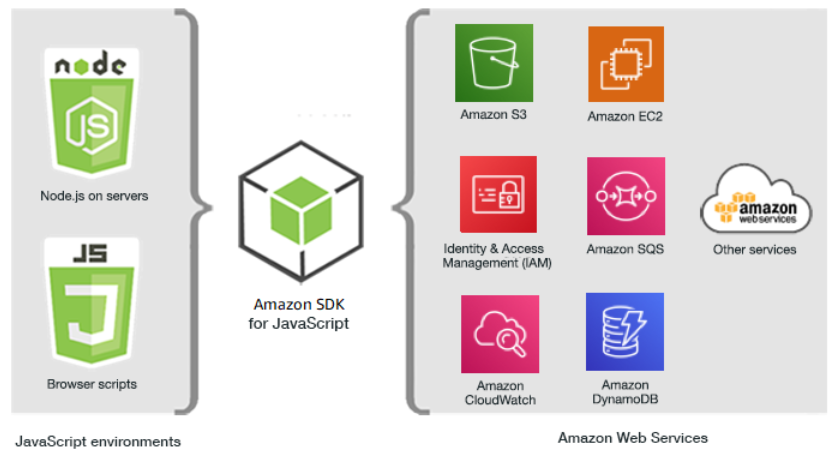
\includegraphics[width=0.8\textwidth]{images/AWSSDK.png}  % Sostituisci 'nome_immagine' con il nome del tuo file immagine e l'estensione
        \caption{The high level rappresentation of the AWS SDK for JavaScript v3 \cite{AWSSDK}}
        \label{fig:AWSSDK}
    \end{figure}
    
    \item \textbf{AWS CDK} 
    
    The AWS Cloud Development Kit (CDK) "is an open-source software development framework for defining cloud infrastructure in code and provisioning it through AWS CloudFormation" \cite{WhatIsTheAWSCDK}. This tool was used in the final phase of the POC design to automate the creation of the stack comprising all the services used.
    
    \item \textbf{AWS IoT Core} 
    
    AWS IoT Core provides the ability to connect IoT devices to AWS cloud services. AWS IoT Core enables the connection of IoT devices to AWS cloud services. It simplifies the integration of IoT devices with other AWS services. This is especially relevant in the automotive industry, where vehicle system ECUs can be viewed as multiple IoT devices. Communication between the device and AWS services can occur in several modes, with the MQTT protocol being the most important for this project. The device can be connected by developing applications that utilize the SDK libraries. Once the data is transmitted, it can be utilized for various purposes such as testing, validation, and analysis. The AWS IoT services, including the IoT Core service, allow for the creation of digital twins of physical IoT devices, known as Thing, and monitoring of traffic on selected MQTT channels. These elements will be explored in greater detail later in the PoC analysis.
    \begin{figure}[h]  % 'h' significa che la figura viene posizionata qui
        \centering
        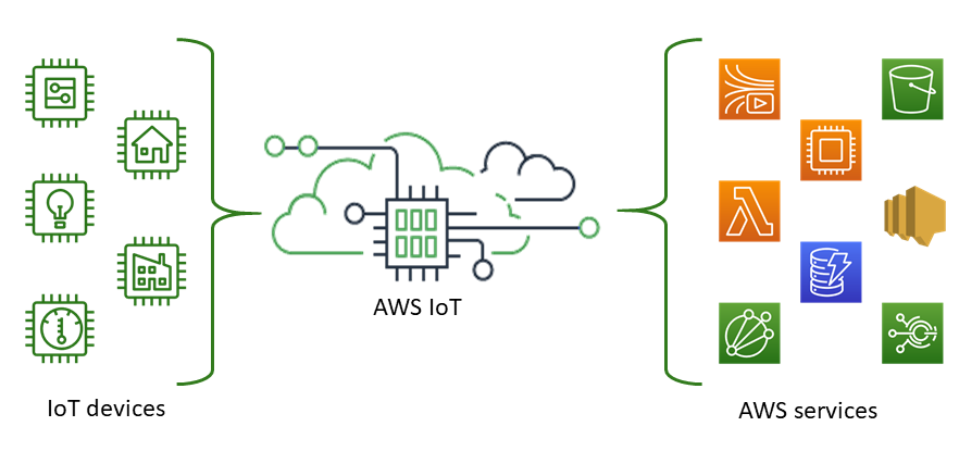
\includegraphics[width=0.8\textwidth]{images/AWSIoTCore.png}  % Sostituisci 'nome_immagine' con il nome del tuo file immagine e l'estensione
        \caption{AWS IoT Core connection system beetween IoT device and AWS service \cite{AWSIoTCore}}
        \label{fig:AWSIoTCore}
    \end{figure}

    \item \textbf{AWS IoT Greengrass}
    
    "AWS IoT Greengrass is an open source Internet of Things (IoT) edge runtime and cloud service that helps you build, deploy and manage IoT applications on devices" \cite{AWSIoTGreengrass}. It is designed to work with intermittent connections and can manage fleets of devices in the field, locally or remotely, using MQTT or other protocols. Once installed, this service can be accessed through the command line. It was utilized in the early stages of project development as an agent to handle updates on the vehicle simulator side. However, this solution will be replaced by a custom solution as explained later.
    
    \item \textbf{AWS IAM}
    
    "AWS Identity and Access Management (IAM) is a web service for securely controlling access to AWS services [...] such as access keys, and permissions that control which AWS resources users and applications can access" \cite{AWSIAM}. IAM is a service that provides a powerful access management mechanism. However, for the purpose of this thesis, only the relevant functionality to the project will be analyzed, specifically IAM's role management capabilities.An IAM role is an identity within AWS that can be assigned specific permissions via permission policies to determine what actions can and cannot be taken. Roles can be assumed by users, applications, or services that do not normally have access to the specific AWS resources. The IAM service also provides another important concept, that of policy, which is an AWS object that, when attached to an identity (including roles) or a resource, enables the creation of permissions and access control to other resources. For example, as explained below, a policy can be attached to the cloud representation of an IoT Core device to enable the connection of the physical dual IoT device or to grant Subscriber or Publisher permissions in a communication via MQTT protocol.
    \item \textbf{AWS Lambda}
    
    AWS Lambda is a computing service that provides the ability to run code without servers. It runs code on a high-performance computing infrastructure and handles administrative tasks related to computing resources autonomously, such as server and operating system management, capacity provisioning, automatic scaling, and logging. It is possible to run code for potentially any type of backend application or service \cite{AWSLambda}. Code can be written directly in Lambda console or imported from the local environment, and it supports several languages, including Python and JavaScript. The Lambda service can also manipulate data from other AWS services or manage tasks with services outside AWS as will be analyzed below.
    \item \textbf{AWS Codepipeline}
    
    AWS CodePipeline is a fully managed continuous delivery service that automates release pipelines for software updates. It enables fast and reliable updates to applications and infrastructure, facilitating the rapid release of new features, iterative development based on feedback, and bug detection through testing every code change. The software release process can be modeled and configured quickly via the stages execution. A stage is a logical unit that creates an isolated environment and allows for the execution of a limited number of concurrent software changes. Each stage contains actions that are executed on application artifacts, such as source code from Codecommit. For instance, as shown in the image \ref{fig:AWSCodepipeline}, it is feasible to establish a software development pipeline that incorporates a codecommit repository as its source stage. This way, a codecommit-related event triggers the pipeline execution which then proceeds to the software build stage. An execution is defined as a series of modifications released from a pipeline.   Each execution represents a set of modifications, such as a merged commit or a manual release of the last commit. Subsequently, the pipeline moves on to the test stage where the desired tests can be launched via Codebuild, and finally delivers the application for production. 
    \begin{figure}[h]  % 'h' significa che la figura viene posizionata qui
        \centering
        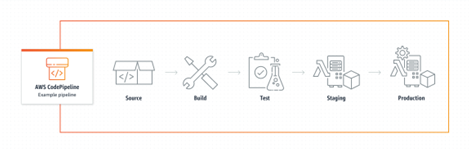
\includegraphics[width=0.8\textwidth]{images/AWSCodepipeline.png}  % Sostituisci 'nome_immagine' con il nome del tuo file immagine e l'estensione
        \caption{An example of a CodePipeline in which some stages are reported \cite{AWSCodepipeline}}
        \label{fig:AWSCodepipeline}
    \end{figure}
    \item \textbf{AWS Codebuild}
    
    AWS CodeBuild is a fully managed build service in the cloud that provides source code compilation, unit testing, and production of executable programs ready for distribution \cite{AWSCodebuild}. CodeBuild provides out-of-the-box configuration of compilation environments for popular programming languages, such as Python. It is also possible to create build platforms for programming languages for which there is no preconfiguration, but in this case it is necessary to leverage multiple AWS services. It is also possible to use codebuild to run tests on application code using for example the pytest tool that allows you to test python code.
    
    \item \textbf{AWS Codecommit}
    
    "AWS CodeCommit is a version control service that enables you to privately store and manage Git repositories in the AWS Cloud" \cite{AWSCodecommit}. This service becomes particularly interesting in the context of multiple services working together, including Lambda, Codepipeline, and Codebuild, because it allows the repository's Git and all its associated events (such as commit and push) to be used to trigger events that can automate various operations, such as triggering a pipeline in Codepipeline. As a result, CodePipelines typically use a CodeCommit repository as their inputo Source stage.
    
    \item \textbf{Amazon S3}
    
    "Amazon Simple Storage Service (Amazon S3) is an object storage service that offers industry-leading scalability, data availability, security, and performance" \cite{AWSamazonS3}. The data saved in the storage is physically placed in multiple locations to ensure the durability of the data even if there is tampering with an item due to the presence of these copies; optionally, it can also be chosen to store the data in a single location to reduce the cost of the service. Amazon S3 can be used for data collection, aggregation, and analysis in many contexts and scenarios, but in the scope of this project, this service is used to store data that is transferred from one stage of the Codepipeline to another. Amazon's Codepipeline service automatically implements this method of output use. However, data stored in S3 from one stage to another can be manipulated through integration with other AWS services, such as Lambda.
    \begin{figure}[h]  % 'h' significa che la figura viene posizionata qui
        \centering
        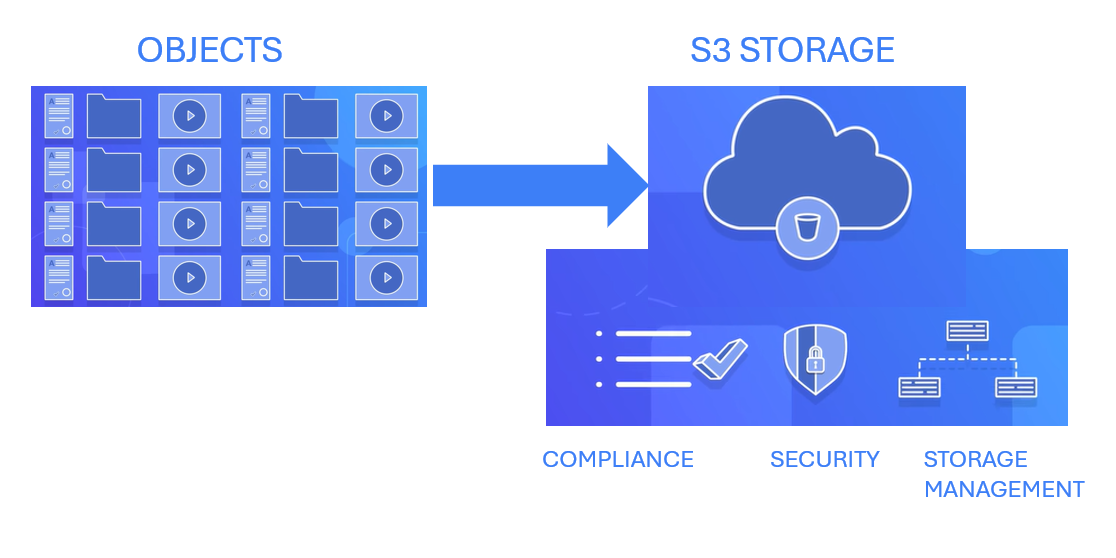
\includegraphics[width=0.8\textwidth]{images/AWSS3.png}  % Sostituisci 'nome_immagine' con il nome del tuo file immagine e l'estensione
        \caption{Amazon S3 high level storing rappresentation}
        \label{fig:AWSS3}
    \end{figure}
    
    \item \textbf{Amazon ECR}
    
    "Amazon Elastic Container Registry (Amazon ECR) is an AWS managed container image registry service that is secure, scalable, and reliable. Amazon ECR supports private repositories with resource-based permissions using AWS IAM. This is so that specified users or Amazon EC2 instances can access [...] container repositories and images" \cite{AmazonECR}. Basically, as shown in the figure \ref{fig:AWSECR}, once the software has been produced and packaged, for example through the use of the CodeBuild service, it can be uploaded to Amazon ECR. The ECR takes care of encrypting the image and controlling access to it, and then automatically manages the entire lifecycle of the image. Once the image is on ECR, it can be used either as an image for local download or through other AWS services. 
    \begin{figure}[h]  % 'h' significa che la figura viene posizionata qui
        \centering
        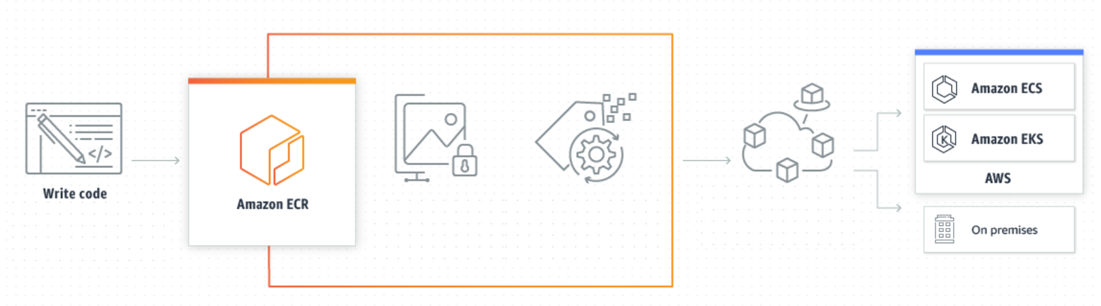
\includegraphics[width=0.8\textwidth]{images/AWSECR.png}  % Sostituisci 'nome_immagine' con il nome del tuo file immagine e l'estensione
        \caption{Example of how Amazon ECR works in production and for pulling images \cite{AWSECR}}
        \label{fig:AWSECR}
    \end{figure}
    
    \item \textbf{EC2}
    
    Amazon Elastic Compute Cloud (Amazon EC2) provides scalable, on-demand computing capacity in the Amazon Web Services (AWS) cloud. With Amazon EC2, users can create and use virtual machines in the cloud, instantiating resources as needed to perform compute operations. Amazon EC2 is a common choice for rapidly deploying applications because it provides an excellent computing resource at a low cost \cite{AWSEC2}, and it is possible to manage networks of different instances of EC2 virtual machines through Amazon Virtual Private Cloud (VPC) and set their relative security, either on a per-instance basis or on an overall network basis. Additionally, it is possible to increase the capacity (scale up) of the instance after creation to handle computationally heavy tasks, such as spikes in website traffic. Conversely, if utilization decreases, capacity can be reduced (scale down). EC2 instances can be launched with Amazon Machine Images (AMIs), which are preconfigured templates containing the necessary components to use the server, including the operating system and additional software. AWS provides pre-built AMIs, but it is also possible to create your own AMIs using containers. Furthermore, it is possible to connect to an EC2 instance through various communication systems, such as using SSH keys provided at the time of instance creation.
    
    \item \textbf{AWS System Manager}
    
    AWS Systems Manager is a service that provides visibility and control of the infrastructure on AWS.  It allows users to view operational data from multiple AWS services and manage the automation of operational tasks across different AWS resources \cite{AWSSM}. The AWS System Manager service is particularly relevant to the project due to its application management capability, namely the Parameter Store. Parameter Store is used to securely store configuration data and secrets, such as passwords, connection strings, and Amazon Machine Image (AMI) identifiers. Values are stored hierarchically by assigning hierarchical names to stored values using the "/" character, while maintaining the uniqueness of the name. For example, names such as Parameters/Parameter1, Parameters/Parameter2 can be used. In addition, it is possible to choose whether to store the data as plain text or encrypted data. Stored data can be retrieved directly from other services, for example, by interacting with Lambdas and SDK code functions.
    
    \item \textbf{Amazon Kinesis Data Streams}
    
    Amazon Kinesis Data Streams is used to collect and process large streams of data records in real time, and eventually route them through other AWS services to various data collection and analysis applications, such as Amazon S3 as it is shown in the image \ref{fig:AmazonKinesis}. "The delay between the time a record is put into the stream and the time it can be retrieved (put-to-get delay) is typically less than 1 second. In other words, a Kinesis Data Streams application can start consuming the data from the stream almost immediately after the data is added" \cite{AWSKinesis}. The Kinesis Data Stream service allows for the selection of specific data based on characteristics through an integrated query system. Additionally, this service can serve as input for lambda functions or to populate databases. 
    \begin{figure}[h]  % 'h' significa che la figura viene posizionata qui
        \centering
        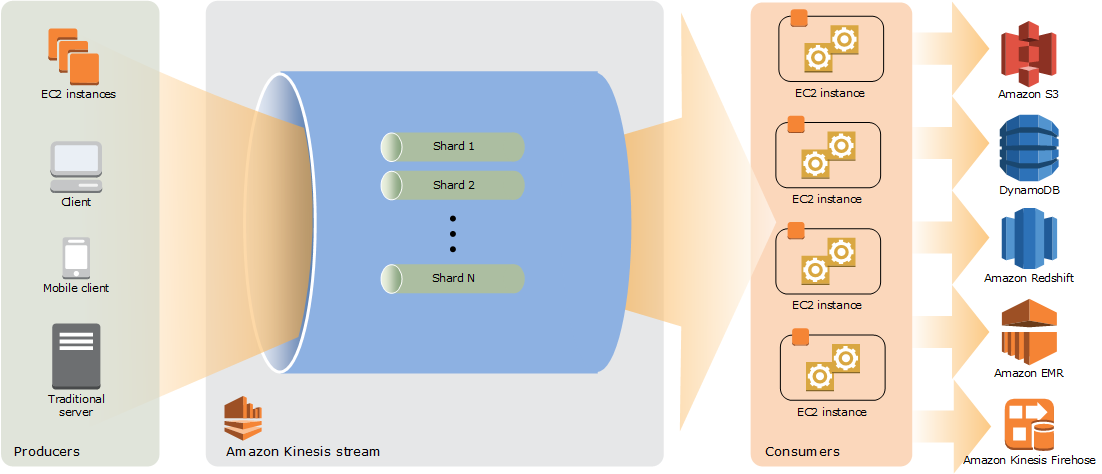
\includegraphics[width=0.8\textwidth]{images/AmazonKinesis.png}  % Sostituisci 'nome_immagine' con il nome del tuo file immagine e l'estensione
        \caption{Illustration of the high-level architecture of Kinesis Data Streams with some examples of services that use the output of the stream. \cite{AmazonKinesis}}
        \label{fig:AmazonKinesis}
    \end{figure}
    
    \item \textbf{Amazon Timestream}
    
    Amazon Timestream is a time-series database that allows you to store and easily analyze large amounts of data stored at regular intervals, ensuring that the time-series data is always encrypted, whether at rest or in transit. This service simplifies the complex process of managing the lifecycle of data by providing storage tiering with an in-memory store for current data and a magnetic store for historical data using Amazon S3 space. The transition of data between these two storage types is enabled through the use of user-configurable policies. The data lifecycle management mechanism makes Amazon Timestream ideal for handling telemetry data from IoT devices, for example. The service also provides a built-in interface for accessing data through a query engine \cite{AWSTimestream}. The Timestrem service also provides an interface for Grafana to view and analyze stored data, which will be explored later.
    
    \item \textbf{DinamoDB}
    
    Amazon DynamoDB is a full-featured NoSQL database service that provides high perfomances both speed and scalability. DynamoDB removes the administrative complexity of running and scaling your distributed database, so there's no need to manage provisioning, hardware setup and configuration, replication, software patching, or cluster sizing. DynamoDB also provides encryption at rest, eliminating the operational costs associated with protecting sensitive data. DynamoDB provides the ability to change the allocation of resources needed to store data in real time to use only the resources required. Additionally, DynamoDB offers on-demand backup functionality for long-term retention and archival purposes, as well as point-in-time recovery to safeguard against accidental write or delete operations. This feature enables users to restore a table to any point within the last 35 days \cite{AWSDynamoDB}. Note that this service was not utilized in the final version of the project, but was considered during development as an alternative for data storage and as a case study for understanding the data storage mechanisms used by AWS services.
    
    \item \textbf{Amazon Cloudwatch}
    
    Amazon CloudWatch is a system to monitor the Amazon Web Services (AWS) resources and the applications running on the infrastructure in real time. With the use of CloudWatch it is possible to collect and track metrics from other AWS services such as Lambda, which are numeric variables that can be measured and analyzed for resources applications \cite{AWSCloudwatch}. Practically this service represents the center for viewing and analyzing logs from the various AWS services in use.
\end{itemize}

All of the previously listed services have been useful, both as an active part in the project's realization and as potential options for the project's implementation, which will be analyzed below. 

After reviewing the various services theoretically, it is now possible to understand a high-level look at how the various services interact with each other.
The interaction system is intricate and consists of two main circuits. The image \ref{fig:AWSDataServices} shows the management of data from the TCU edge device in the first part. The data is sent to the cloud via the IoT Core thing, inserted into a Kinesis channel, and then sent to a Timestream database in relevant tables.
\begin{figure}[h]  % 'h' significa che la figura viene posizionata qui
    \centering
    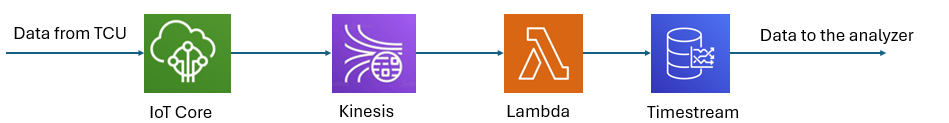
\includegraphics[width=1\textwidth]{images/AWS_data_services.png}  % Sostituisci 'nome_immagine' con il nome del tuo file immagine e l'estensione
    \caption{The high level rappresentation of the ASW services for the data managing}
    \label{fig:AWSDataServices}
\end{figure}

\begin{figure}[h]  % 'h' significa che la figura viene posizionata qui
    \centering
    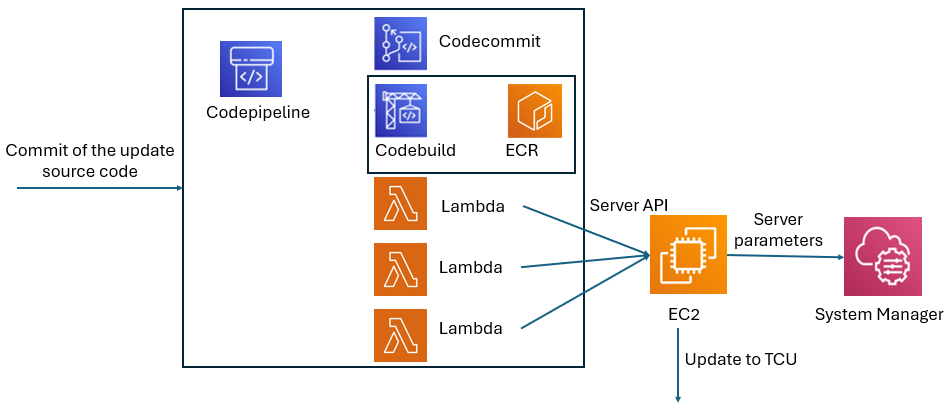
\includegraphics[width=1\textwidth]{images/AWS_update_services.png}  % Sostituisci 'nome_immagine' con il nome del tuo file immagine e l'estensione
    \caption{The high level rappresentation of the ASW services for the update managing}
    \label{fig:AWSUpdateServices}
\end{figure}
During the second part of the service interaction shown in the image \ref{fig:AWSUpdateServices}, the system consists of a Codepipeline that can be triggered by a Codecommit event acting as a source. The pipeline includes a build phase via Codebuild, which can utilize images from ECR registries, followed by three phases consisting of Lambda functions. The pipeline interacts with a server located on an EC2 instance, which stores its key information in the parameter Stor of the System Manager service.

The components of the cloud structure may appear separate, indeed there is no actual interaction between data management services and update management services. However, the TCU device serves as the point of connection. It continuously sends data to the cloud, which can be analyzed, and receives updates. This process can continue indefinitely.

The following section provides a detailed analysis of the PoC structure, covering the edge device, cloud infrastructure, their connection, and data analysis system.
\lstdefinestyle{yaml}{
     basicstyle=\color{red}\footnotesize,
     rulecolor=\color{black},
     string=[s]{'}{'},
     stringstyle=\color{red},
     comment=[l]{:},
     commentstyle=\color{black},
     morecomment=[l]{-}
 }
 
\chapter{Proof Of Concept} \label{ch:proofOfConcept}

This chapter explores the Proof of Concept (PoC) phase within the context of the thesis, aiming to validate the feasibility and efficacy of implementing SDV technologies. The main objective of this chapter is to translate theoretical concepts into concrete results, demonstrating the practical application of SDV in real-world situations. Through the PoC, we aim to confirm the fundamental principles and features of SDV, including its potential impact on vehicle performance, user experience, and overall safety.

The multifaceted nature of SDV requires a structured approach to its implementation, taking into account factors such as standardized hardware, cloud integration, and over-the-air (OTA) updates. To achieve this, a PoC was designed to address these components individually and holistically, ensuring a seamless integration that aligns with the envisioned paradigm shift in automotive manufacturing. Furthermore, this chapter aims to demonstrate the collaborative efforts with industry-leading technologies and platforms, highlighting the strategic partnerships forged with key players in the automotive and software development sectors. By aligning with renowned entities, the PoC aims to leverage their expertise, technologies, and frameworks, thereby enhancing the robustness and scalability of the SDV ecosystem.

Test and Validation are the concluding phases of this chapter, where the Proof of Concept is subjected to real-world scenarios. A demonstration involving a Raspberry Pi (RPi) serves as a tangible validation of the implemented SDV functionalities. This section serves as the litmus test, affirming the seamless orchestration of SDV within the envisioned architecture.

The exploration of the POC begins by detailing the services and technologies offered by Amazon Web Services (AWS) in the IoT, data management, and automotive essential for project implementation.

\section{AWS Used Services}
As discussed in previous chapters, the development of SDV technology requires a cloud infrastructure to handle server-side operations. AWS is a leading player in the cloud world, and therefore an ideal alternative for the advancement of SDV, as well as an active partner in the implementation of technologies that contribute to the creation of a publicly available SDV for all. The following discussion introduces and analyzes, via AWS documentation the key tools for successful Proof of Concept (POC) implementation.

\begin{itemize}
    \item AWS CLI: The AWS Command Line Interface (CLI) is an essential tool for developing with AWS services. t allows interaction with AWS services from the command line of a local PC, enabling the creation of infrastructure and management of properties from the command line.
    \item AWS Boto: Boto is an AWS SDK made for Python. A software Development Kit (SDK), more generally, is a set of creation tools specifically for developing and running software in a single platform. It includes resources such as documentation, examples, and APIs to facilitate faster application development. Boto basically works as an interface for applications that need to interact with and take advantage of the services provided by AWS. The AWS SDK for JavaScript v3 is another example of an SDK for JavaScript that works basically in the same way.
    \begin{figure}[h]  % 'h' significa che la figura viene posizionata qui
        \centering
        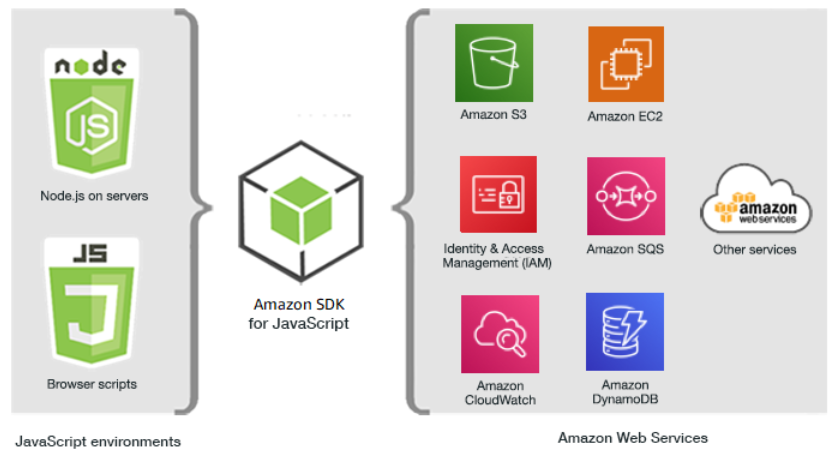
\includegraphics[width=0.8\textwidth]{images/AWSSDK.png}  % Sostituisci 'nome_immagine' con il nome del tuo file immagine e l'estensione
        \caption{The high level rappresentation of the AWS SDK for JavaScript v3 \cite{AWSSDK}}
        \label{fig:AWSSDK}
    \end{figure}
    \item AWS CDK: The AWS Cloud Development Kit (CDK) "is an open-source software development framework for defining cloud infrastructure in code and provisioning it through AWS CloudFormation" \cite{WhatIsTheAWSCDK}. This tool was used in the final phase of the POC design to automate the creation of the stack comprising all the services used.
    \item AWS IoT Core: AWS IoT Core provides the ability to connect IoT devices to AWS cloud services. AWS IoT Core enables the connection of IoT devices to AWS cloud services. It simplifies the integration of IoT devices with other AWS services. This is especially relevant in the automotive industry, where vehicle system ECUs can be viewed as multiple IoT devices. Communication between the device and AWS services can occur in several modes, with the MQTT protocol being the most important for this project. The device can be connected by developing applications that utilize the SDK libraries. Once the data is transmitted, it can be utilized for various purposes such as testing, validation, and analysis.
    \begin{figure}[h]  % 'h' significa che la figura viene posizionata qui
        \centering
        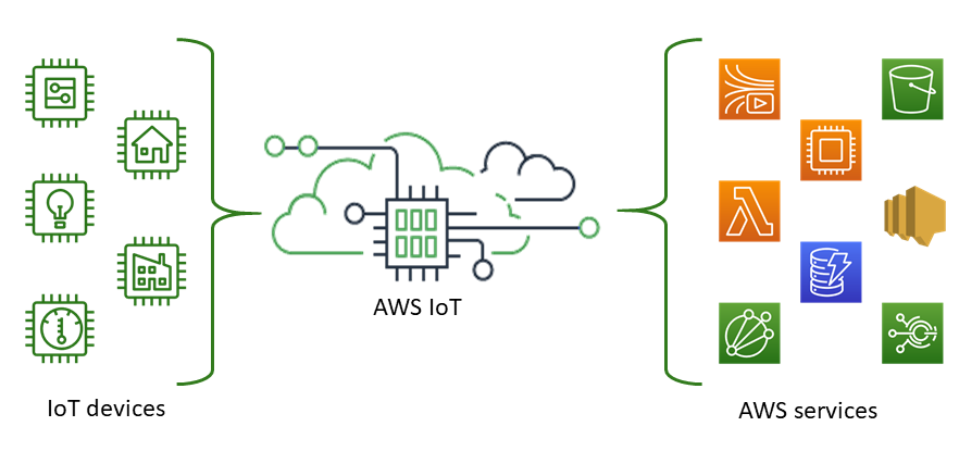
\includegraphics[width=0.8\textwidth]{images/AWSIoTCore.png}  % Sostituisci 'nome_immagine' con il nome del tuo file immagine e l'estensione
        \caption{AWS IoT Core connection system beetween IoT device and AWS service \cite{AWSIoTCore}}
        \label{fig:AWSIoTCore}
    \end{figure}
    \item AWS IoT Greengrass: "AWS IoT Greengrass is an open source Internet of Things (IoT) edge runtime and cloud service that helps you build, deploy and manage IoT applications on devices" \cite{AWSIoTGreengrass}. It is designed to work with intermittent connections and can manage fleets of devices in the field, locally or remotely, using MQTT or other protocols. Once installed, this service can be accessed through the command line. It was utilized in the early stages of project development as an agent to handle updates on the vehicle simulator side. However, this solution will be replaced by a custom solution as explained later.
    \item AWS IAM: "AWS Identity and Access Management (IAM) is a web service for securely controlling access to AWS services [...] such as access keys, and permissions that control which AWS resources users and applications can access" \cite{AWSIAM}. IAM is a service that provides a powerful access management mechanism. However, for the purpose of this thesis, only the relevant functionality to the project will be analyzed, specifically IAM's role management capabilities.An IAM role is an identity within AWS that can be assigned specific permissions via permission policies to determine what actions can and cannot be taken. Roles can be assumed by users, applications, or services that do not normally have access to the specific AWS resources. The IAM service also provides another important concept, that of policy, which is an AWS object that, when attached to an identity (including roles) or a resource, enables the creation of permissions and access control to other resources. For example, as explained below, a policy can be attached to the cloud representation of an IoT Core device to enable the connection of the physical dual IoT device or to grant Subscriber or Publisher permissions in a communication via MQTT protocol.
    \item AWS Lambda: AWS Lambda is a computing service that provides the ability to run code without servers. It runs code on a high-performance computing infrastructure and handles administrative tasks related to computing resources autonomously, such as server and operating system management, capacity provisioning, automatic scaling, and logging. It is possible to run code for potentially any type of backend application or service \cite{AWSLambda}. Code can be written directly in Lambda console or imported from the local environment, and it supports several languages, including Python and JavaScript. The Lambda service can also manipulate data from other AWS services or manage tasks with services outside AWS as will be analyzed below.
    \item AWS Codepipeline: AWS CodePipeline is a fully managed continuous delivery service that automates release pipelines for software updates. It enables fast and reliable updates to applications and infrastructure, facilitating the rapid release of new features, iterative development based on feedback, and bug detection through testing every code change. The software release process can be modeled and configured quickly via the stages execution. A stage is a logical unit that creates an isolated environment and allows for the execution of a limited number of concurrent software changes. Each stage contains actions that are executed on application artifacts, such as source code from Codecommit. For instance, as shown in the image \ref{fig:AWSCodepipeline}, it is feasible to establish a software development pipeline that incorporates a codecommit repository as its source stage. This way, a codecommit-related event triggers the pipeline execution which then proceeds to the software build stage. An execution is defined as a series of modifications released from a pipeline.   Each execution represents a set of modifications, such as a merged commit or a manual release of the last commit. Subsequently, the pipeline moves on to the test stage where the desired tests can be launched via Codebuild, and finally delivers the application for production. 
    \begin{figure}[h]  % 'h' significa che la figura viene posizionata qui
        \centering
        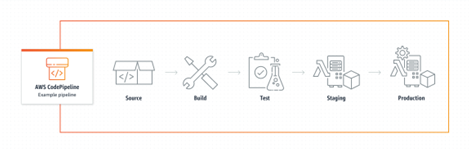
\includegraphics[width=0.8\textwidth]{images/AWSCodepipeline.png}  % Sostituisci 'nome_immagine' con il nome del tuo file immagine e l'estensione
        \caption{An example of a CodePipeline in which some stages are reported \cite{AWSCodepipeline}}
        \label{fig:AWSCodepipeline}
    \end{figure}
    \item AWS Codebuild: AWS CodeBuild is a fully managed build service in the cloud that provides source code compilation, unit testing, and production of executable programs ready for distribution \cite{AWSCodebuild}. CodeBuild provides out-of-the-box configuration of compilation environments for popular programming languages, such as Python. It is also possible to create build platforms for programming languages for which there is no preconfiguration, but in this case it is necessary to leverage multiple AWS services. It is also possible to use codebuild to run tests on application code using for example the pytest tool that allows you to test python code.
    \item AWS Codecommit: "AWS CodeCommit is a version control service that enables you to privately store and manage Git repositories in the AWS Cloud" \cite{AWSCodecommit}. This service becomes particularly interesting in the context of multiple services working together, including Lambda, Codepipeline, and Codebuild, because it allows the repository's Git and all its associated events (such as commit and push) to be used to trigger events that can automate various operations, such as triggering a pipeline in Codepipeline. As a result, CodePipelines typically use a CodeCommit repository as their inputo Source stage.
    \item Amazon S3: "Amazon Simple Storage Service (Amazon S3) is an object storage service that offers industry-leading scalability, data availability, security, and performance" \cite{AWSamazonS3}. The data saved in the storage is physically placed in multiple locations to ensure the durability of the data even if there is tampering with an item due to the presence of these copies; optionally, it can also be chosen to store the data in a single location to reduce the cost of the service. Amazon S3 can be used for data collection, aggregation, and analysis in many contexts and scenarios, but in the scope of this project, this service is used to store data that is transferred from one stage of the Codepipeline to another. Amazon's Codepipeline service automatically implements this method of output use. However, data stored in S3 from one stage to another can be manipulated through integration with other AWS services, such as Lambda.
    \begin{figure}[h]  % 'h' significa che la figura viene posizionata qui
        \centering
        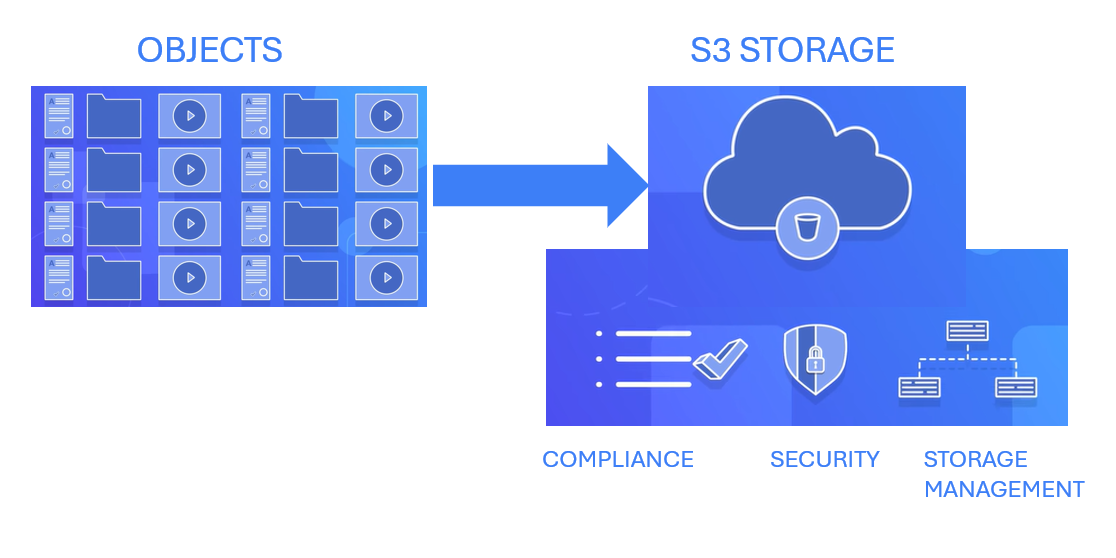
\includegraphics[width=0.8\textwidth]{images/AWSS3.png}  % Sostituisci 'nome_immagine' con il nome del tuo file immagine e l'estensione
        \caption{Amazon S3 high level storing rappresentation}
        \label{fig:AWSS3}
    \end{figure}
    \item Amazon ECR: "Amazon Elastic Container Registry (Amazon ECR) is an AWS managed container image registry service that is secure, scalable, and reliable. Amazon ECR supports private repositories with resource-based permissions using AWS IAM. This is so that specified users or Amazon EC2 instances can access [...] container repositories and images" \cite{AmazonECR}. Basically, as shown in the figure \ref{fig:AWSECR}, once the software has been produced and packaged, for example through the use of the CodeBuild service, it can be uploaded to Amazon ECR. The ECR takes care of encrypting the image and controlling access to it, and then automatically manages the entire lifecycle of the image. Once the image is on ECR, it can be used either as an image for local download or through other AWS services. 
    \begin{figure}[h]  % 'h' significa che la figura viene posizionata qui
        \centering
        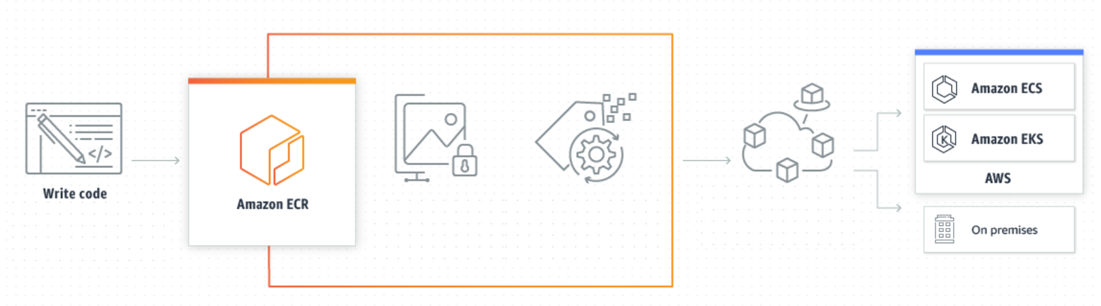
\includegraphics[width=0.8\textwidth]{images/AWSECR.png}  % Sostituisci 'nome_immagine' con il nome del tuo file immagine e l'estensione
        \caption{Example of how Amazon ECR works in production and for pulling images \cite{AWSECR}}
        \label{fig:AWSECR}
    \end{figure}
    \item EC2: Amazon Elastic Compute Cloud (Amazon EC2) provides scalable, on-demand computing capacity in the Amazon Web Services (AWS) cloud. With Amazon EC2, users can create and use virtual machines in the cloud, instantiating resources as needed to perform compute operations. Amazon EC2 is a common choice for rapidly deploying applications because it provides an excellent computing resource at a low cost \cite{AWSEC2}, and it is possible to manage networks of different instances of EC2 virtual machines through Amazon Virtual Private Cloud (VPC) and set their relative security, either on a per-instance basis or on an overall network basis. Additionally, it is possible to increase the capacity (scale up) of the instance after creation to handle computationally heavy tasks, such as spikes in website traffic. Conversely, if utilization decreases, capacity can be reduced (scale down). EC2 instances can be launched with Amazon Machine Images (AMIs), which are preconfigured templates containing the necessary components to use the server, including the operating system and additional software. AWS provides pre-built AMIs, but it is also possible to create your own AMIs using containers. Furthermore, it is possible to connect to an EC2 instance through various communication systems, such as using SSH keys provided at the time of instance creation.
    \item AWS System Manager: AWS Systems Manager is a service that provides visibility and control of the infrastructure on AWS.  It allows users to view operational data from multiple AWS services and manage the automation of operational tasks across different AWS resources \cite{AWSSM}. The AWS System Manager service is particularly relevant to the project due to its application management capability, namely the Parameter Store. Parameter Store is used to securely store configuration data and secrets, such as passwords, connection strings, and Amazon Machine Image (AMI) identifiers. Values are stored hierarchically by assigning hierarchical names to stored values using the "/" character, while maintaining the uniqueness of the name. For example, names such as Parameters/Parameter1, Parameters/Parameter2 can be used. In addition, it is possible to choose whether to store the data as plain text or encrypted data. Stored data can be retrieved directly from other services, for example, by interacting with Lambdas and SDK code functions.
    \item Amazon Kinesis Data Streams: Amazon Kinesis Data Streams is used to collect and process large streams of data records in real time, and eventually route them through other AWS services to various data collection and analysis applications, such as Amazon S3 as it is shown in the image \ref{fig:AmazonKinesis}. "The delay between the time a record is put into the stream and the time it can be retrieved (put-to-get delay) is typically less than 1 second. In other words, a Kinesis Data Streams application can start consuming the data from the stream almost immediately after the data is added" \cite{AWSKinesis}.
    \begin{figure}[h]  % 'h' significa che la figura viene posizionata qui
        \centering
        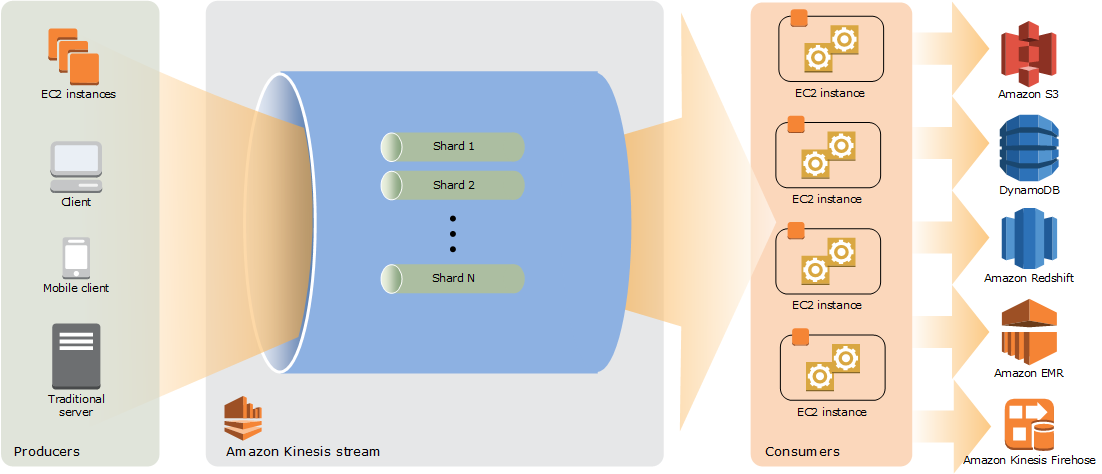
\includegraphics[width=0.8\textwidth]{images/AmazonKinesis.png}  % Sostituisci 'nome_immagine' con il nome del tuo file immagine e l'estensione
        \caption{Illustration of the high-level architecture of Kinesis Data Streams with some examples of services that use the output of the stream. \cite{AmazonKinesis}}
        \label{fig:AmazonKinesis}
    \end{figure}
    \item Amazon Timestream: Amazon Timestream is a time-series database that allows you to store and easily analyze large amounts of data stored at regular intervals, ensuring that the time-series data is always encrypted, whether at rest or in transit. This service simplifies the complex process of managing the lifecycle of data by providing storage tiering with an in-memory store for current data and a magnetic store for historical data using Amazon S3 space. The transition of data between these two storage types is enabled through the use of user-configurable policies. The data lifecycle management mechanism makes Amazon Timestream ideal for handling telemetry data from IoT devices, for example. The service also provides a built-in interface for accessing data through a query engine \cite{AWSTimestream}. The Timestrem service also provides an interface for Grafana to view and analyze stored data, which will be explored later.
    \item DinamoDB: Amazon DynamoDB is a full-featured NoSQL database service that provides high perfomances both speed and scalability. DynamoDB removes the administrative complexity of running and scaling your distributed database, so there's no need to manage provisioning, hardware setup and configuration, replication, software patching, or cluster sizing. DynamoDB also provides encryption at rest, eliminating the operational costs associated with protecting sensitive data. DynamoDB provides the ability to change the allocation of resources needed to store data in real time to use only the resources required. Additionally, DynamoDB offers on-demand backup functionality for long-term retention and archival purposes, as well as point-in-time recovery to safeguard against accidental write or delete operations. This feature enables users to restore a table to any point within the last 35 days \cite{AWSDynamoDB}. Note that this service was not utilized in the final version of the project, but was considered during development as an alternative for data storage and as a case study for understanding the data storage mechanisms used by AWS services.
    \item Amazon Cloudwatch: Amazon CloudWatch is a system to monitor the Amazon Web Services (AWS) resources and the applications running on the infrastructure in real time. With the use of CloudWatch it is possible to collect and track metrics from other AWS services such as Lambda, which are numeric variables that can be measured and analyzed for resources applications \cite{AWSCloudwatch}. Practically this service represents the center for viewing and analyzing logs from the various AWS services in use.
\end{itemize}

All of the previously listed services have been useful, both as an active part in the project's realization and as potential options for the project's implementation, which will be analyzed below. The analysis of the POC will start with a description of the project's design, followed by an analysis of how the various services are actively involved in the project, and then an analysis of the interaction between the various elements that make up the architecture.

\section{Architectural design}
This section delves into the heart of the project implementation, starting with a high-level view of the various systems that make up its realization and transitioning to a visualization of the interactions between the various elements.

The study and analysis of the Software Defined Vehicle case study revealed that three fundamental elements were essential to create a concrete example of SDV implementation:
\begin{itemize}
    \item TCU simulator: The TCU simulator is a system that replicates the basic functions of a telematic control unit (TCU). The system has the capability to send data packets and receive updates from a cloud server structure.
    \item Cloud infrastructure: The cloud infrastructure must be capable of managing both the data from the TCU and the update function.
    \item Data viewer:  The data viewer is a platform that enables the visualization of manipulated and processed data in a manner that clearly displays changes in data behavior resulting from variations in the data and updates to the TCU.
\end{itemize}

With these three elements, a practical implementation made it possible to achieve what should happen in an SDV: having a vehicle system capable of updating itself via Over The Air updates. To support this implementation, it was necessary to use the services previously mentioned for creating the cloud infrastructure through the services made available by AWS.

Now, let's look at the components of the POC in detail through a high-level architectural representation of the previously introduced elements and a more detailed analysis of the code that compose them.

\subsection{TCU Simulator}
Come telematic control unit (TCU) in questo progetto si intende un sistema harware in grado di generare in qualche modo dei dati provenienti da una o più sottosistemi dei un eventuale veicolo, raccoglierli, per poi essere pronti per essere inviati all'esterno del veicolo. Per prendere familiarità con questo tipo di strutture e per dare forma al progetto di esempio, è stato necessario simulare una TCU in modo tale ceh fosse il più vicino possibile ad un sistema reale, senza però avere la disponibilità di un veicolo vero e proprio. Quindi riducendo ai minimi termini il concetto è stata presa come punto di arrivo di TCU una scheda raspberry pi che fosse in grado di generare dati telemetrici.

\begin{figure}[h]  % 'h' significa che la figura viene posizionata qui
    \centering
    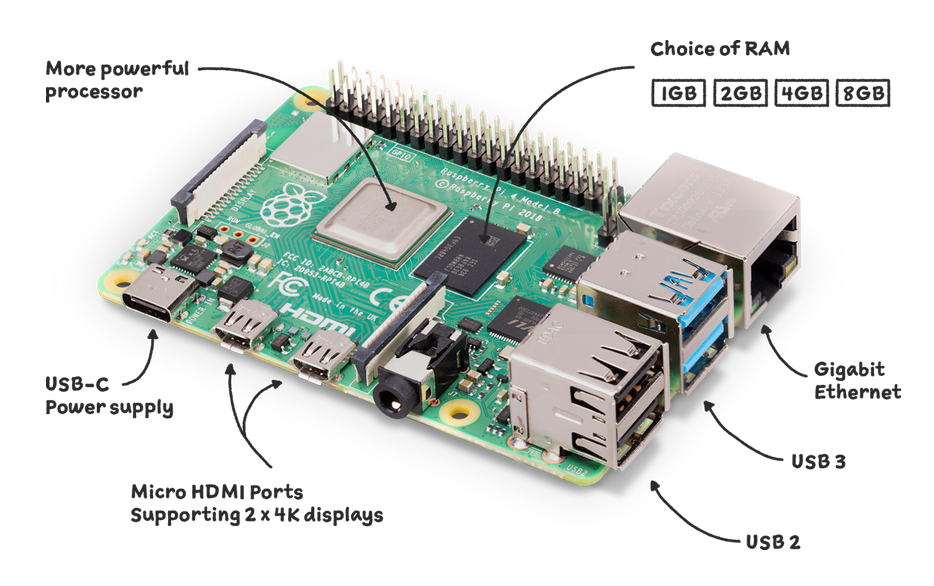
\includegraphics[width=0.8\textwidth]{images/raspberrypi.png}  % Sostituisci 'nome_immagine' con il nome del tuo file immagine e l'estensione
    \caption{Illustration of a RaspberryPi board with its periferics \cite{raspberrypi}}
    \label{fig:raspberrypi}
\end{figure}

Come riportato in figura \ref{fig:raspberrypi} una RaspberryPi è una scheda contenente tutto il necessario per funzionare come un sistema indipendente a cui possono essere attaccate diverse periferiche, per questo motivo rappresenta l'ideale astrazione di una TCU general porpous necessaria per la realizzazione del caso di studio del SOC del SDV.

Prima di mettere mano alla raspberry però è stata necessaria una fase priliminare di realizzazione del progetto su macchina virtuale, il ciò ha facilitato notevolmente lo sviluppo e il test del codice scritto.

Il simulatore, nelle sue diverse fasi di sviluppo è stato pensato composto da 4 diverse componenti software, ognuna caratterizzata dalle proprie funzionalità:
\begin{itemize}
    \item Elemento responsabile del collegamento al cloud server per l'invio di dati telematici;
    \item Elemento per il collegamento al server cloud per l'aggiornamento dell'unità telematica;
    \item Elemento per la generazione dei dati telematici;
    \item Elemento per l'update locale dell'unità telematica.
\end{itemize}

Questi 4 elementi sono orchestrati da uno script esterno che gestisce l'avvio dell'unità di simulazione tramite linea di comando. 
Analizzando nel dettaglio questi 4 elementi, il primo elemento in ordine cronologico preso come studio è stato l'elemnto responsabile al collegamento del sistema con l'infrastruttura cloud tramite protocllo MQTT. Questo elemento, ovviamente ha richiesto come azione preliminare la presenza di un servizio attivo di IoT Core lato cloud che come analizzeremo in seguito genera un certificato con annessa coppia di chiavi pubblica e privata per garantire l'identità del dispositivo. La disscussione relativa all'infrastruttura cloud verrà analizzata in seguito. 

Per permettere il collegamento alla piattaforma cloud analizziamo il seguente codice \ref{lst:MQTTConnection} viene lanciato uno script Python che tramite la funzione AWSIoTMQTTClient della libreria AWSIoTPythonSDK.MQTTLib crea il collegamento, se possibile, con il server IoT Core per poi potergli inviare i dati. In particolare con mqttc = AWSIoTMQTTClient(VIN) viene creato il Clien MQTT, mentre con mqttc.configureEndpoint(ENDPOINT, 8883) is configured the host name and port number the client tries to connect to e con mqttc.configureCredentials(ROOT_CA_FILEPATH, PRIVATE_KEY_FILEPATH, CERT_FILEPATH) vengono forniti e configurati i certificati di autenticazione. Da notare che i file sono infatti salvati in locale sul dispositivo e devono essere accessibili dallo script di collegamento. Il collwgamento MQTT verrà fatto sul topic device/{VIN}/telemetry, quindi il servizio AWS che sarà collegato al topic tramite le opportune policies, come vedremo in seguito sarà in grado di ricevere i dati inviati.

\begin{lstlisting}[language=Python, caption={MQTT connection to the IoT Core AWS service}, label=lst:MQTTConnection]
    from AWSIoTPythonSDK.MQTTLib import AWSIoTMQTTClient

    certificate_path="./Permanent/Certificates/"

    def telemetry_handler(): #Function that manage the telemetry data sending to IoTCore via mqtt protocol
        global mqttc
        global connection_event
        #Thing connection
        VIN = "HawkbitDevice001"  ##This is the Thing name
        ENDPOINT = "a1tbrylx7y3p3t-ats.iot.eu-west-1.amazonaws.com"
        CERT_FILEPATH = f"{certificate_path}{VIN}.cert.pem"
        PRIVATE_KEY_FILEPATH = f"{certificate_path}{VIN}.private.key"
        ROOT_CA_FILEPATH = f"{certificate_path}root-CA.crt"
        mqttc = AWSIoTMQTTClient(VIN)
        # Make sure you use the correct region!
        mqttc.configureEndpoint(ENDPOINT, 8883)
        mqttc.configureCredentials(ROOT_CA_FILEPATH, PRIVATE_KEY_FILEPATH, CERT_FILEPATH)
        # Connect to the gateway
        if mqttc.connect():
            print("Connected to IoT core. Now the device sends its telemetry every 1 seconds")
            connection_event.set() #Send connected signal to the main
            publish_topic = f"device/{VIN}/telemetry"
\end{lstlisting}

Il secondo elemento in analisi utilizzato per la realizzazione del simulatore è l'elemento che permette la connessione con il OTA Server per permettere il riconoscimento e il downolad degli aggiornamenti OTA. Questo è stato possibile tramite l'utilizzo come base di partenza del "Device Simulator" messo a disposizione in maniera aperta dal Hawkbit stesso. In questo caso si tratta di uno script Java che sfrutta l'interfaccia del Server Hawkbit pr collegarsi al server e rimanere in ascolto per attendere la presenza di aggiornamenti dedicarti al dispositivco stesso.
Il collegamento viene fatto in automatico all'avvio del codice tramite le Simulation properties impostate, in particolare ai fini del progetto sperimentale il nome del device viene impostato in modo statico in SimulationProperties.java come private String name = "HawkbitDevice001"; mentre l'ip del server a cui connettersi viene preso come input in DeviceSimulator.java da System.setProperty("spring.rabbitmq.host", newHost); in cui newHost contiene l'informazione presa come input.
\begin{lstlisting}[language=Java, caption={Hawbit Device simulator source code}, label=lst:HawkbitDeviceSimulator]
    private static long getOverallRead(final CloseableHttpResponse response, final MessageDigest md, final String url) throws IOException {
        long overallread = 0L;
        String[] urlParts = url.split("/");
        File downloadFolder = new File("./TCU/downloads");
        if (!downloadFolder.exists()) { //If "Download" folder doesn't exist
            boolean created = downloadFolder.mkdirs();
            if (!created) {
                System.err.println("Error in the directory creation!");
            }
        }
        File downloadFile = new File("./TCU/downloads/"+urlParts[10]);
        try (FileOutputStream outputStream = new FileOutputStream(downloadFile);
        final BufferedOutputStream bos = new BufferedOutputStream(new DigestOutputStream(outputStream, md))) {
            try (BufferedInputStream bis = new BufferedInputStream(response.getEntity().getContent())) {
                byte[] buffer = new byte[8192]; //byte dimension from createBuffer of ByteStream.class
                int bytesRead;
                while ((bytesRead = bis.read(buffer)) != -1) {
                    bos.write(buffer, 0, bytesRead); //Here only for the md hash correctness.
                    overallread += bytesRead;
                }
            }
        }
        return overallread;
    }
\end{lstlisting}
In seguito, come mostrato nelle parti salienti del codice sorgente di DeviceSimulatorUpdater.java, nel momento in cui il dispositivo riceve un segnale di download, dopo aver eseguito diversi controlli di sicurezza, questo viene avviato e i dati ricevuti vengono inseriti nella cartella specifica "./TCU/downloads/" tramite l'utilizzo di uno stream che prende i dati in arrivo dal collegamento e li inserisce nella cartella selezionata, con il nome del file ricavato dall'url di download. 

in un primo momento come un elemento che potesse interagire con l'utente: sostanzialmente il simulatore si occupava di fare 3 cose:
\begin{itemize}
    \item Catturare gli input da utente;
    \item Raccogliere i dati ed inviarli al cloud;
    \item Riconoscere la presenza di aggiornamenti, quindi restartare il sistema con l'aggiornamento avvenuto.
\end{itemize}
SPIEGARE OGNI ELEMENTO CON CODICE ANNESSO

PARLARE DEL FATTO CHE L'IMPLEMENTAZIONE DEL CODICE è STATA FATTA IN TRE FASI: PRIMA CON UNINTERFACCIA E POCHI DATI GENERATI, POI SENZA INTERFACCIA E UNA ATTIVAZIONE DIRETTA DELL'INVIO DI DATI CON PYTHON POI CON C++ POI CON C. SPIEGARE OGNI SINGOLO ELEMENTO DELLA TCU FACENDO RIFERIMENTO ANCHE ALLA SCHEDA ED EVENTUALMENTE DARE LA COMPOSIZIONE DI UN GUADRO CHE PIANO PIANO SI COSTRUISCE PER CREARE L'INTERA TCU
\subsection{Cloud Infrastructure}
\subsection{Data Viewer}

\section{Test and Validation}
\subsection{RPi demo}
\chapter{Conclding Remarks} \label{ch:concldingRemarks}
In this final chapter, first of all, the results obtained with the test demo of the project developed during the course are presented, then an analysis is made in relation to the objectives proposed by the thesis, evaluating what has been achieved and the future work that can be related to the project.

This chapter aims to be a conclusion for the thesis work done, both from the descriptive side by providing a summary of the work done, and from the practical side of project development, but also with the purpose of providing open options for furthering the project. The SDV technologies are very young and there are many development ideas. In addition, as an open project with the objective of creating a standard for the entire automotive industry, there are many opportunities for collaboration.

Let's start the description with the conclusions gathered with the final test demo of the project on RaspberryPi.

\section{Test and Validation on RaspberryPi}
To create the test demo, a RaspberryPi 4 board was used, with an architecture based on Cortex-A72, a processor from the ARM family. This device was found to be the best solution for simulating a modern automotive TCU physical system.

First of all, it was necessary to instantiate the cloud stacks of AWS services so that the supporting cloud structure was operational and ready to interact with the board. Once the necessary certificates for communication with the cloud platform had been obtained, it was possible to insert the communication scripts on the RaspberryPi.

Once the script was started, the communication was successful and the generated data arrived at the cloud server ready to be analyzed, as shown in the image \ref{fig:RaspberryPiDemo}. The only difference compared to the simulations performed on a local virtual machine was the time it took to receive the data. In particular, in the case of the Raspberry Pi, there was a delay in sending data, although it was almost imperceptible and acceptable for the purposes of the test.
\begin{figure}[h]  % 'h' significa che la figura viene posizionata qui
    \centering
    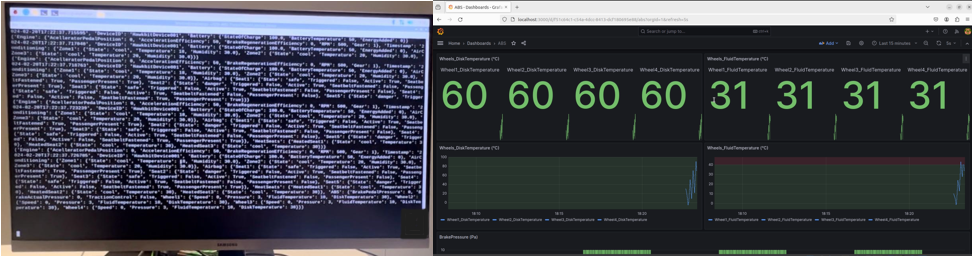
\includegraphics[width=0.9\textwidth]{images/RaspberryPiDemo.png}  % Sostituisci 'nome_immagine' con il nome del tuo file immagine e l'estensione
    \caption{Comunication between the RaspberryPi board and the Grafana server via the AWS cloud services}
    \label{fig:RaspberryPiDemo}
\end{figure}

At this point, it was possible to start the update using the AWS CodePipeline service. In particular, once the update process was started on the pipeline, it was able to correctly contact the Hawkbit server where the TCU simulator was already present to start the update. 
Also in this case, it was necessary to wait a few more seconds for the update to be received on the device, but once this happened, the Raspberry Pi was able to interrupt the flow, receive the update, and restart the system with the updated features. 
As shown in the figure \ref{fig:RaspberryPiDemoUpdate}, the update was also detected by the data analysis server. Specifically, both the Python updates, which showed a drastic change in the data sent, and the update compiled in C, which caused an interruption in the sending of data, as expected by the update itself were launched on the demo board.

The presentation of test demos on the RaspberryPi board was useful from several points of view and showed the following characteristics
\begin{itemize}
    \item The ability of the system to communicate through the MQTT protocol across different connection networks.
    \item The capability of the software simulator to be used on different platforms, including ARM.
    \item The flexibility to adapt the cloud infrastructure to different conditions, whether it is a virtual machine or a physical board.
    \item Correct implementation of the pipeline capable of computing update projects written in compiled languages.
\end{itemize}
\begin{figure}[h]  % 'h' significa che la figura viene posizionata qui
    \centering
    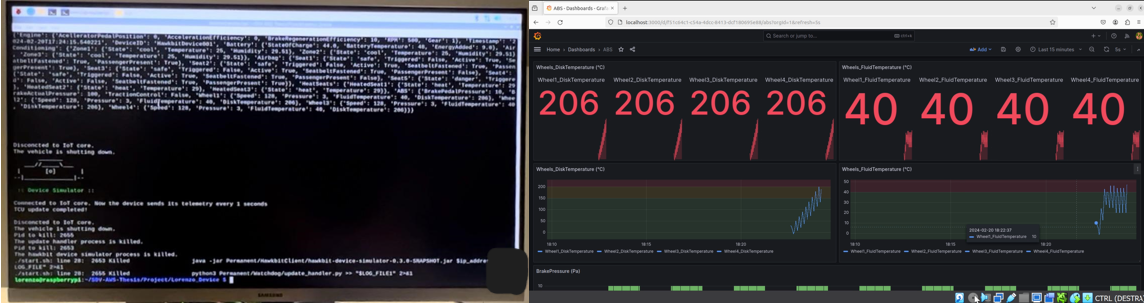
\includegraphics[width=0.9\textwidth]{images/RaspberryPiDemoUpdate.png}  % Sostituisci 'nome_immagine' con il nome del tuo file immagine e l'estensione
    \caption{Update to the RaspberryPi board and Grafana data after the update}
    \label{fig:RaspberryPiDemoUpdate}
\end{figure}

\section{Contribution Recaps}
The aim of the thesis was to show the innovations introduced by the Software Defined Vehicle technology, which is capable of completely revolutionizing the automotive industry. This result was achieved thanks to the support of the partner company, which provided the necessary resources to study, understand and analyze the cloud services offered by AWS, but also to put them into practice in the implementation of the project, which included technologies currently used by several companies in the automotive sector.

The SDV represents a true innovation in the automotive field, as it would allow the industry to move forward in creating more efficient and safer vehicles. In addition, it would open the door to a different and innovative development and production method that could significantly reduce production costs and times, thereby reducing the waste of necessary resources.

The thesis has certainly achieved its objectives, but let's now evaluate whether the objectives of the project, which was created to give a practical demonstration of the cooperation between the various elements involved in the SDV, have been achieved.

\subsection{Are the PoC goals being met?}
One of the main objectives of the proof of concept was to demonstrate how the cloud infrastructure composed of services provided by AWS could support the development of the SDV by using its resources. Certainly, this objective was fully achieved with the use of more than one pipeline responsible for managing updates. In particular, both the updates in Python language, easily portable from one platform to another, and the updates in compiled languages, more targeted and specific to each platform, but also more optimized and closer to the real use case, were successfully carried out.

Another important goal of the work was to be able to bring together different technologies to support the creation of the infrastructure. Specifically, the project succeeded in making AWS cloud services work with the Hawkbit system (already under development in several automotive companies) for managing the deployment of updates, and with Grafana services for data analysis. Achieving this goal made it possible to make the most of the technologies offered at the lowest possible cost to the company, obtaining a true ecosystem that is as open as possible.

As a final goal of the project, we can identify the need to introduce general purpose systems to support the development of the SDV. Also in this case, as seen before, the demo on the Raspberry Pi board showed that it can interact masterfully with different general purpose platforms and make the best use of the available resources.

In conclusion, the results obtained at the beginning of the implementation can be considered as achieved. However, it is important to emphasize that the PoC was a demonstration example, still in its early stages as far as actual production is concerned. The remaining points, deliberately left open due to limited resources, will be addressed below.

\section{Future Works}
Now the open aspects for the future development of the project are analyzed. In consideration of the nature of the work, some aspects were deliberately neglected in order to achieve a complete and functional result. If there had been an ambition to create a fully functional product on a real vehicle ready for use, not even a small part of the project could have been achieved with the available resources. Now let's talk about future work.

\subsection{Transform the poc in a product}
To transform the proof of concept into a real product, usable in an automotive system capable of producing vehicles, it is necessary to cover three different steps: interfacing with a real vehicle to study the operational dynamics of a real TCU with all the subsystems that compose it, delving into the detailed analysis of the free software used such as Hawkbit, and managing additional elements of the vehicle such as machine learning or cockpit applications. A brief overview of each of these future works is given below.
\begin{enumerate}
    \item Making the system usable with a real vehicle is essential to creating a market-ready commercial product. A real vehicle is made up of dozens, if not hundreds, of subsystems interconnected at various levels, and the management of all the data produced may be slightly different from what is seen in the PoC. The telemetry systems of real vehicles contain security systems that prevent direct connection to each individual subsystem, for example through firewalls; this is another aspect to consider when building a real product.
    \item Another fundamental aspect for the creation of a concrete product is the in-depth analysis of the operational dynamics of the free software used in the development of the infrastructure. In particular, with regard to the Hawkbit server, in the PoC, after a not too detailed analysis of the various components, it was decided to use a pre-built Docker image. This made it easier to manage the elements, since everything was ready, but limited the freedom of customization. To fully exploit the potential of these technologies, it will be essential to fully customize the software used, as happens in real companies.
    \item Last, but not least, is the adaptability of the Software Defined Vehicle system to additional elements of the vehicle, such as machine learning systems for decision making or cockpit systems. For the PoC to become a usable product in reality, it is essential that it is fully integrated into the vehicle. Therefore, it is inconceivable that there are systems in the vehicle itself that do not interface with the SDV system, especially if they are other systems strictly related to IT, such as those mentioned above.  
\end{enumerate}

In conclusion, the full integration of the PoC with a real vehicle represents an essential phase in the development of the technologies covered in the thesis. This would allow vehicles to be transformed into fully upgradeable devices, thus contributing to the improvement of efficiency and safety, fundamental elements in the automotive sector.
\bibliographystyle{IEEEtran}
\bibliography{bibliography}

%if appendixes are needed, uncomment the following lines
%\appendix
%\appendixpage
%\include{appendixA}
%\include{appendixB}
\end{document}

